\documentclass{article}

\usepackage{a4}
\usepackage{amsmath}
\usepackage{amssymb}
\usepackage{ctex}
\usepackage{booktabs}
\usepackage{graphicx}
\usepackage{subfigure}
\usepackage{subcaption}
\usepackage{float}
\usepackage{hyperref}
\usepackage{xurl}
\usepackage{enumitem}
\usepackage{array}
\usepackage{longtable}
\usepackage{multirow}
\usepackage{fvextra}

\hypersetup{colorlinks=true,linkcolor=black,urlcolor=blue,citecolor=black}
\setlist[itemize]{nosep,leftmargin=1.8em}
\setlist[enumerate]{nosep,leftmargin=1.8em}
\captionsetup{font=small}
\RecustomVerbatimEnvironment{verbatim}{Verbatim}{
  breaklines=true,
  breakanywhere=true,
  fontsize=\small
}

\title{计算机组成原理 \\ 实验4 ALU复现与改进}
\author{鲁昕宁 2414015}
\date{\today}

\begin{document}

\maketitle
\begin{center}
    \url{https://github.com/SidneyLu/Computer-Organization-and-Design-NKU-CS/tree/master/lab4}
\end{center}

\newpage

\section{实验目标}
参考实验指导手册第四次的ALU实验，完成对ALU的改进：
\begin{enumerate}
    \item 原来的12位独热编码控制信号压缩为4位
    \item 增加至少三个指令：一个比较指令，一个位运算指令，一个加载指令
\end{enumerate}

\section{实验原理}
本实验新增了三条指令，采用4位编码（4'b1100~4'b1110）进行控制。新增的三条指令分别为：
\begin{enumerate}
    \item \textbf{SEQ（Set if Equal，比较相等）：} 比较指令，用于判断两个操作数是否相等。当 \texttt{src1 == src2} 时，结果置 1，否则置 0。该指令通过复用加法器实现，将 \texttt{src1 - src2} 的结果是否为 0 作为判断依据。
    \item \textbf{XNOR（Exclusive NOR，按位同或）：} 位运算指令，是异或（XOR）的取反操作。当两对应位相同时结果为 1，不同时结果为 0，即 \texttt{~(src1 \textasciicircum{} src2)}。
    \item \textbf{LLI（Load Lower Immediate，低位加载）：} 加载指令，将 16 位立即数扩展后写入目标寄存器，即 \texttt{\{16'd0, src2[15:0]\}}，与 LUI（高位加载）指令互为补充。
\end{enumerate}
修改后的控制信号译码表：
\begin{verbatim}
    // 0000: ADD   0001: SUB   0010: SLT   0011: SLTU
    // 0100: AND   0101: NOR   0110: OR    0111: XOR
    // 1000: SLL   1001: SRL   1010: SRA   1011: LUI
    // 1100: SEQ   1101: XNOR  1110: LLI   1111: 保留
\end{verbatim}

\begin{figure}[h]
    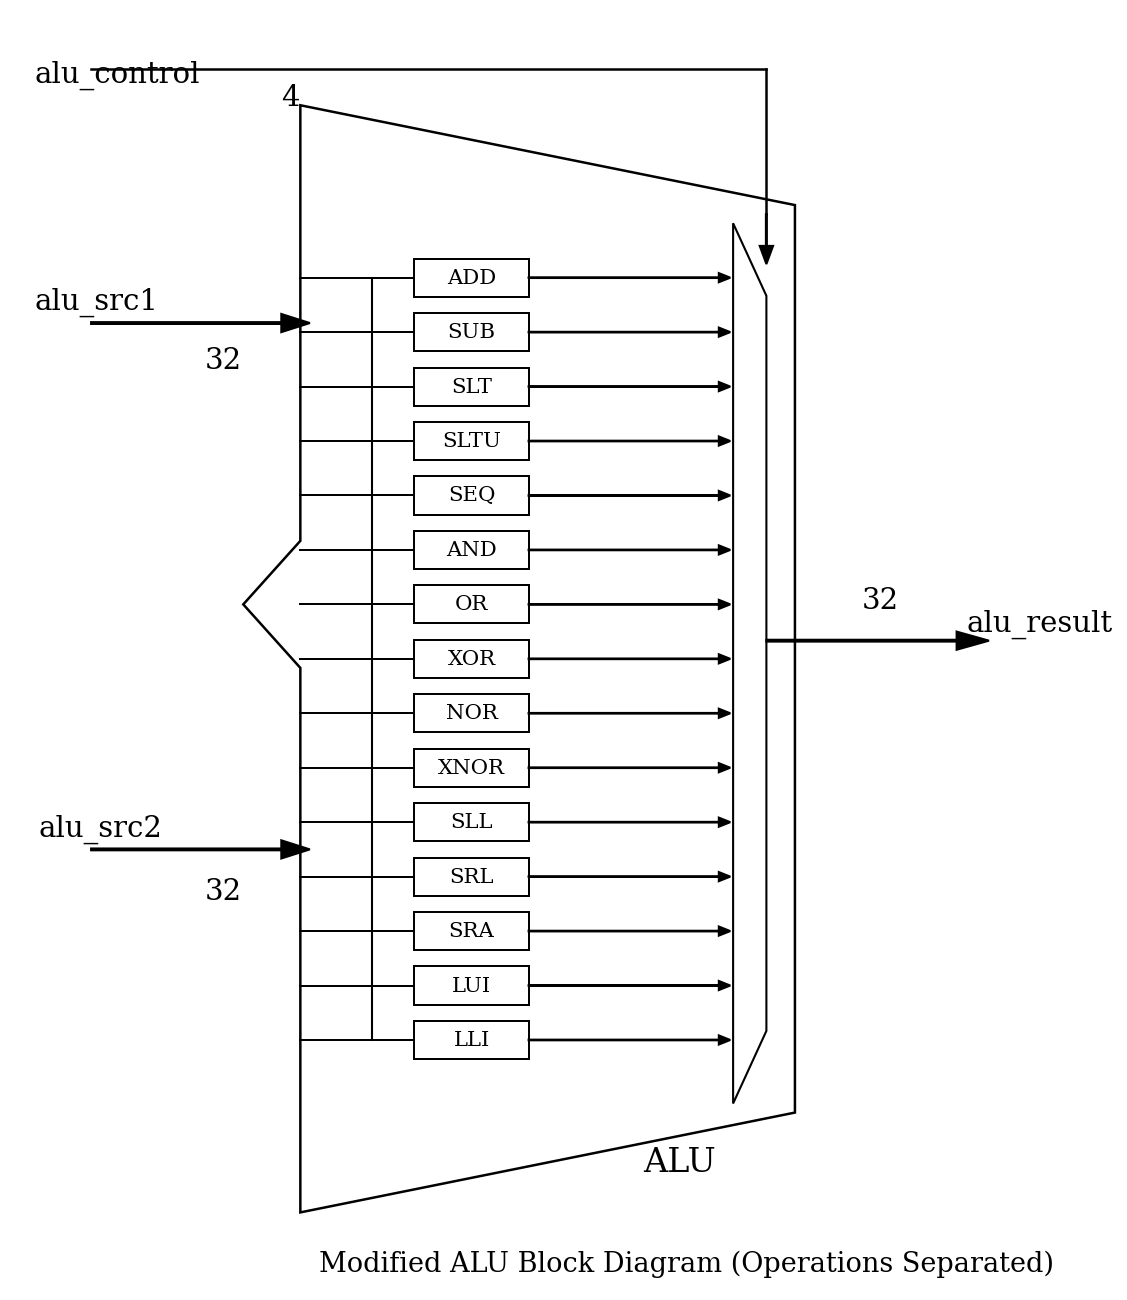
\includegraphics[width=0.5\textwidth]{alu.png}
\end{figure}

\section{实验过程}

\subsection{源码修改}
\begin{verbatim}
`timescale 1ns / 1ps
//*************************************************************************
//   > 文件名: alu.v
//   > 描述  ：ALU模块，使用4位编码控制，可做15种操作
//   > 作者  : LOONGSON
//   > 日期  : 2016-04-14
//*************************************************************************
module alu(
    input  [3 :0] alu_control,  // ALU控制信号（4位编码）
    input  [31:0] alu_src1,     // ALU操作数1,为补码
    input  [31:0] alu_src2,     // ALU操作数2，为补码
    output [31:0] alu_result    // ALU结果
    );

    // ALU控制信号（4位编码）
    // 0000: ADD   0001: SUB   0010: SLT   0011: SLTU
    // 0100: AND   0101: NOR   0110: OR    0111: XOR
    // 1000: SLL   1001: SRL   1010: SRA   1011: LUI
    // 1100: SEQ   1101: XNOR  1110: LLI   1111: 保留
    wire alu_add;   //加法操作
    wire alu_sub;   //减法操作
    wire alu_slt;   //有符号比较，小于置位，复用加法器做减法
    wire alu_sltu;  //无符号比较，小于置位，复用加法器做减法
    wire alu_and;   //按位与
    wire alu_nor;   //按位或非
    wire alu_or;    //按位或
    wire alu_xor;   //按位异或
    wire alu_sll;   //逻辑左移
    wire alu_srl;   //逻辑右移
    wire alu_sra;   //算术右移
    wire alu_lui;   //高位加载
    wire alu_seq;   //比较相等，相等置位（新增比较运算）
    wire alu_xnor;  //按位同或（新增位运算）
    wire alu_lli;   //低位加载（新增加载运算）

    assign alu_add  = (alu_control == 4'h0);
    assign alu_sub  = (alu_control == 4'h1);
    assign alu_slt  = (alu_control == 4'h2);
    assign alu_sltu = (alu_control == 4'h3);
    assign alu_and  = (alu_control == 4'h4);
    assign alu_nor  = (alu_control == 4'h5);
    assign alu_or   = (alu_control == 4'h6);
    assign alu_xor  = (alu_control == 4'h7);
    assign alu_sll  = (alu_control == 4'h8);
    assign alu_srl  = (alu_control == 4'h9);
    assign alu_sra  = (alu_control == 4'ha);
    assign alu_lui  = (alu_control == 4'hb);
    assign alu_seq  = (alu_control == 4'hc);
    assign alu_xnor = (alu_control == 4'hd);
    assign alu_lli  = (alu_control == 4'he);

    wire [31:0] add_sub_result;
    wire [31:0] slt_result;
    wire [31:0] sltu_result;
    wire [31:0] seq_result;
    wire [31:0] and_result;
    wire [31:0] nor_result;
    wire [31:0] or_result;
    wire [31:0] xor_result;
    wire [31:0] xnor_result;
    wire [31:0] sll_result;
    wire [31:0] srl_result;
    wire [31:0] sra_result;
    wire [31:0] lui_result;
    wire [31:0] lli_result;

    assign and_result = alu_src1 & alu_src2;      // 与结果为两数按位与
    assign or_result  = alu_src1 | alu_src2;      // 或结果为两数按位或
    assign nor_result = ~or_result;               // 或非结果为或结果按位取反
    assign xor_result = alu_src1 ^ alu_src2;      // 异或结果为两数按位异或
    assign xnor_result= ~(alu_src1 ^ alu_src2);   // 同或结果为异或结果按位取反
    assign lui_result = {alu_src2[15:0], 16'd0};  // 立即数装载结果为立即数移位至高半字节
    assign lli_result = {16'd0, alu_src2[15:0]};  // 低位加载，低16位写入立即数

//-----{加法器}begin
//add,sub,slt,sltu均使用该模块
    wire [31:0] adder_operand1;
    wire [31:0] adder_operand2;
    wire        adder_cin     ;
    wire [31:0] adder_result  ;
    wire        adder_cout    ;
    wire        adder_use_sub ;
    assign adder_use_sub = ~(alu_add);
    assign adder_operand1 = alu_src1; 
    assign adder_operand2 = adder_use_sub ? ~alu_src2 : alu_src2;
    assign adder_cin      = adder_use_sub; //减法需要cin
    adder adder_module(
    .operand1(adder_operand1),
    .operand2(adder_operand2),
    .cin     (adder_cin     ),
    .result  (adder_result  ),
    .cout    (adder_cout    )
    );

    //加减结果
    assign add_sub_result = adder_result;

    //slt结果
    //adder_src1[31] adder_src2[31] adder_result[31]
    //       0             1           X(0或1)       "正-负"，显然小于不成立
    //       0             0             1           相减为负，说明小于
    //       0             0             0           相减为正，说明不小于
    //       1             1             1           相减为负，说明小于
    //       1             1             0           相减为正，说明不小于
    //       1             0           X(0或1)       "负-正"，显然小于成立
    assign slt_result[31:1] = 31'd0;
    assign slt_result[0]    = (alu_src1[31] & ~alu_src2[31]) | (~(alu_src1[31]^alu_src2[31]) & adder_result[31]);

    //sltu结果
    //对于32位无符号数比较，相当于33位有符号数（{1'b0,src1}和{1'b0,src2}）的比较，最高位0为符号位
    //故，可以用33位加法器来比较大小，需要对{1'b0,src2}取反,即需要{1'b0,src1}+{1'b1,~src2}+cin
    //但此处用的为32位加法器，只做了运算:                             src1   +    ~src2   +cin
    //32位加法的结果为{adder_cout,adder_result},则33位加法结果应该为{adder_cout+1'b1,adder_result}
    //对比slt结果注释，知道，此时判断大小属于第二三种情况，即源操作数1符号位为0，源操作数2符号位为0
    //结果的符号位为1，说明小于，即adder_cout+1'b1为2'b01，即adder_cout为0
    assign sltu_result = {31'd0, ~adder_cout};
    
    //seq结果
    assign seq_result = {31'd0, (adder_result == 32'd0)};
//-----{加法器}end

//-----{移位器}begin
    // 移位分三步进行，
    // 第一步根据移位量低2位即[1:0]位做第一次移位，
    // 第二步在第一次移位基础上根据移位量[3:2]位做第二次移位，
    // 第三步在第二次移位基础上根据移位量[4]位做第三次移位。
    wire [4:0] shf;
    assign shf = alu_src1[4:0];
    wire [1:0] shf_1_0;
    wire [1:0] shf_3_2;
    assign shf_1_0 = shf[1:0];
    assign shf_3_2 = shf[3:2];
    
     // 逻辑左移
    wire [31:0] sll_step1;
    wire [31:0] sll_step2;
    assign sll_step1 = {32{shf_1_0 == 2'b00}} & alu_src2                   // 若shf[1:0]="00",不移位
                     | {32{shf_1_0 == 2'b01}} & {alu_src2[30:0], 1'd0}     // 若shf[1:0]="01",左移1位
                     | {32{shf_1_0 == 2'b10}} & {alu_src2[29:0], 2'd0}     // 若shf[1:0]="10",左移2位
                     | {32{shf_1_0 == 2'b11}} & {alu_src2[28:0], 3'd0};    // 若shf[1:0]="11",左移3位
    assign sll_step2 = {32{shf_3_2 == 2'b00}} & sll_step1                  // 若shf[3:2]="00",不移位
                     | {32{shf_3_2 == 2'b01}} & {sll_step1[27:0], 4'd0}    // 若shf[3:2]="01",第一次移位结果左移4位
                     | {32{shf_3_2 == 2'b10}} & {sll_step1[23:0], 8'd0}    // 若shf[3:2]="10",第一次移位结果左移8位
                     | {32{shf_3_2 == 2'b11}} & {sll_step1[19:0], 12'd0};  // 若shf[3:2]="11",第一次移位结果左移12位
    assign sll_result = shf[4] ? {sll_step2[15:0], 16'd0} : sll_step2;     // 若shf[4]="1",第二次移位结果左移16位

    // 逻辑右移
    wire [31:0] srl_step1;
    wire [31:0] srl_step2;
    assign srl_step1 = {32{shf_1_0 == 2'b00}} & alu_src2                   // 若shf[1:0]="00",不移位
                     | {32{shf_1_0 == 2'b01}} & {1'd0, alu_src2[31:1]}     // 若shf[1:0]="01",右移1位,高位补0
                     | {32{shf_1_0 == 2'b10}} & {2'd0, alu_src2[31:2]}     // 若shf[1:0]="10",右移2位,高位补0
                     | {32{shf_1_0 == 2'b11}} & {3'd0, alu_src2[31:3]};    // 若shf[1:0]="11",右移3位,高位补0
    assign srl_step2 = {32{shf_3_2 == 2'b00}} & srl_step1                  // 若shf[3:2]="00",不移位
                     | {32{shf_3_2 == 2'b01}} & {4'd0, srl_step1[31:4]}    // 若shf[3:2]="01",第一次移位结果右移4位,高位补0
                     | {32{shf_3_2 == 2'b10}} & {8'd0, srl_step1[31:8]}    // 若shf[3:2]="10",第一次移位结果右移8位,高位补0
                     | {32{shf_3_2 == 2'b11}} & {12'd0, srl_step1[31:12]}; // 若shf[3:2]="11",第一次移位结果右移12位,高位补0
    assign srl_result = shf[4] ? {16'd0, srl_step2[31:16]} : srl_step2;    // 若shf[4]="1",第二次移位结果右移16位,高位补0
 
    // 算术右移
    wire [31:0] sra_step1;
    wire [31:0] sra_step2;
    assign sra_step1 = {32{shf_1_0 == 2'b00}} & alu_src2                                 // 若shf[1:0]="00",不移位
                     | {32{shf_1_0 == 2'b01}} & {alu_src2[31], alu_src2[31:1]}           // 若shf[1:0]="01",右移1位,高位补符号位
                     | {32{shf_1_0 == 2'b10}} & {{2{alu_src2[31]}}, alu_src2[31:2]}      // 若shf[1:0]="10",右移2位,高位补符号位
                     | {32{shf_1_0 == 2'b11}} & {{3{alu_src2[31]}}, alu_src2[31:3]};     // 若shf[1:0]="11",右移3位,高位补符号位
    assign sra_step2 = {32{shf_3_2 == 2'b00}} & sra_step1                                // 若shf[3:2]="00",不移位
                     | {32{shf_3_2 == 2'b01}} & {{4{sra_step1[31]}}, sra_step1[31:4]}    // 若shf[3:2]="01",第一次移位结果右移4位,高位补符号位
                     | {32{shf_3_2 == 2'b10}} & {{8{sra_step1[31]}}, sra_step1[31:8]}    // 若shf[3:2]="10",第一次移位结果右移8位,高位补符号位
                     | {32{shf_3_2 == 2'b11}} & {{12{sra_step1[31]}}, sra_step1[31:12]}; // 若shf[3:2]="11",第一次移位结果右移12位,高位补符号位
    assign sra_result = shf[4] ? {{16{sra_step2[31]}}, sra_step2[31:16]} : sra_step2;    // 若shf[4]="1",第二次移位结果右移16位,高位补符号位
//-----{移位器}end

    // 选择相应结果输出
    assign alu_result = (alu_add|alu_sub) ? add_sub_result[31:0] : 
                        alu_slt           ? slt_result :
                        alu_sltu          ? sltu_result :
                        alu_and           ? and_result :
                        alu_nor           ? nor_result :
                        alu_or            ? or_result  :
                        alu_xor           ? xor_result :
                        alu_xnor          ? xnor_result:
                        alu_sll           ? sll_result :
                        alu_srl           ? srl_result :
                        alu_sra           ? sra_result :
                        alu_lui           ? lui_result :
                        alu_seq           ? seq_result :
                        alu_lli           ? lli_result :
                        32'd0;
endmodule
\end{verbatim}

\subsection{仿真脚本与波形}
\begin{verbatim}
    `timescale 1ns / 1ps

module tb_alu;
    reg  [3:0]  alu_control;
    reg  [31:0] alu_src1;
    reg  [31:0] alu_src2;
    wire [31:0] alu_result;
    integer errors;

    alu u_alu (
        .alu_control(alu_control),
        .alu_src1   (alu_src1),
        .alu_src2   (alu_src2),
        .alu_result (alu_result)
    );

    task run_case;
        input [255:0] name;
        input [3:0]   op;
        input [31:0]  src1;
        input [31:0]  src2;
        input [31:0]  expected;
        begin
            alu_control = op;
            alu_src1    = src1;
            alu_src2    = src2;
            #1;
            if (alu_result !== expected) begin
                errors = errors + 1;
                $display("[FAIL] %0s op=0x%0h src1=0x%08h src2=0x%08h got=0x%08h exp=0x%08h",
                         name, op, src1, src2, alu_result, expected);
            end else begin
                $display("[PASS] %0s result=0x%08h", name, alu_result);
            end
        end
    endtask

    initial begin
        errors = 0;
        alu_control = 4'h0;
        alu_src1 = 32'd0;
        alu_src2 = 32'd0;
        #5;

        // 0x0 ADD
        run_case("ADD basic",        4'h0, 32'd1,          32'd2,          32'd3);
        run_case("ADD wrap",         4'h0, 32'hffff_ffff,  32'd1,          32'h0000_0000);

        // 0x1 SUB
        run_case("SUB basic",        4'h1, 32'd5,          32'd7,          32'hffff_fffe);

        // 0x2 SLT (signed)
        run_case("SLT -1<1",         4'h2, 32'hffff_ffff,  32'd1,          32'd1);
        run_case("SLT 5<-3",         4'h2, 32'd5,          32'hffff_fffd,  32'd0);

        // 0x3 SLTU (unsigned)
        run_case("SLTU 1<2",         4'h3, 32'd1,          32'd2,          32'd1);
        run_case("SLTU FFFF<1",      4'h3, 32'hffff_ffff,  32'd1,          32'd0);

        // 0x4 AND
        run_case("AND",              4'h4, 32'h55aa_ff00,  32'h0f0f_0f0f,  32'h050a_0f00);

        // 0x5 NOR
        run_case("NOR",              4'h5, 32'h55aa_ff00,  32'h0f0f_0f0f,  32'ha050_00f0);

        // 0x6 OR
        run_case("OR",               4'h6, 32'h55aa_ff00,  32'h0f0f_0f0f,  32'h5faf_ff0f);

        // 0x7 XOR
        run_case("XOR",              4'h7, 32'h55aa_ff00,  32'h0f0f_0f0f,  32'h5aa5_f00f);

        // 0x8 SLL (shift amount = src1[4:0])
        run_case("SLL by 4",         4'h8, 32'd4,          32'h0000_0011,  32'h0000_0110);

        // 0x9 SRL
        run_case("SRL by 4",         4'h9, 32'd4,          32'hf000_0000,  32'h0f00_0000);

        // 0xA SRA
        run_case("SRA by 4",         4'ha, 32'd4,          32'hf000_0000,  32'hff00_0000);

        // 0xB LUI
        run_case("LUI",              4'hb, 32'd0,          32'h1234_5678,  32'h5678_0000);

        // 0xC SEQ
        run_case("SEQ equal",        4'hc, 32'h1234_5678,  32'h1234_5678,  32'd1);
        run_case("SEQ not equal",    4'hc, 32'h1234_5678,  32'h1234_5670,  32'd0);

        // 0xD XNOR
        run_case("XNOR",             4'hd, 32'h55aa_ff00,  32'h0f0f_0f0f,  32'ha55a_0ff0);

        // 0xE LLI
        run_case("LLI",              4'he, 32'd0,          32'h1234_5678,  32'h0000_5678);

        // 0xF reserved/default
        run_case("RESERVED->0",      4'hf, 32'h89ab_cdef,  32'h0123_4567,  32'h0000_0000);

        if (errors == 0)
            $display("\n=== ALU TEST PASS ===");
        else
            $display("\n=== ALU TEST FAIL: %0d errors ===", errors);

        $finish;
    end
endmodule
\end{verbatim}

\begin{figure}[h]
    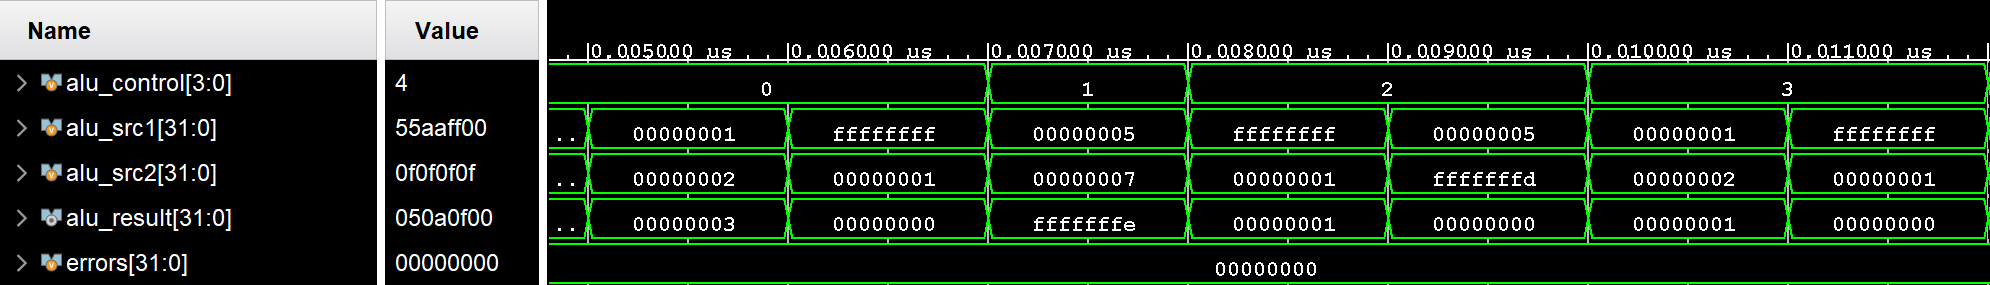
\includegraphics[width=\textwidth]{sim1.png}
    \caption{ALU仿真波形1}
\end{figure}

\begin{figure}[h]
    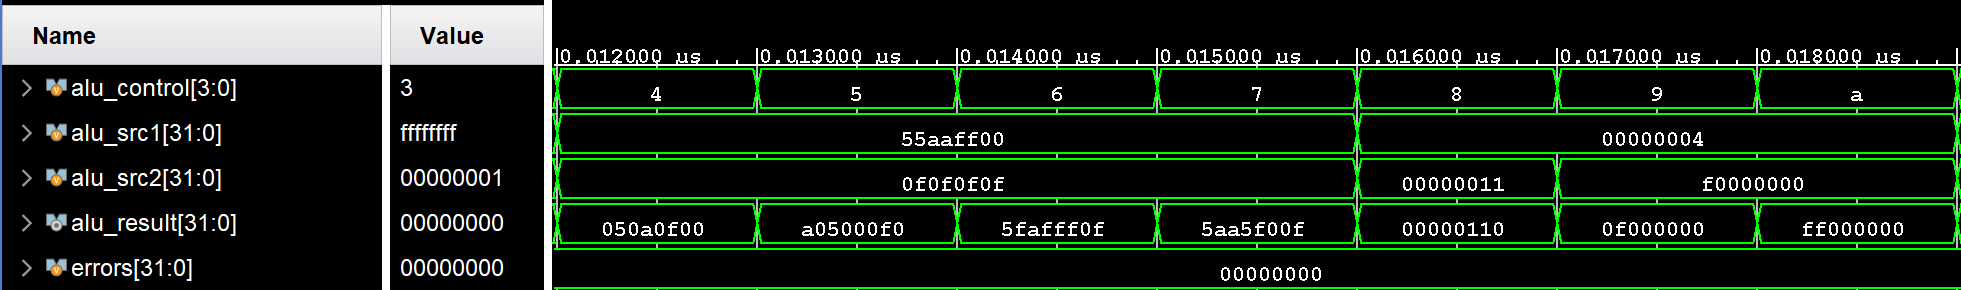
\includegraphics[width=\textwidth]{sim2.png}
    \caption{ALU仿真波形2}
\end{figure}

\begin{figure}[h]
    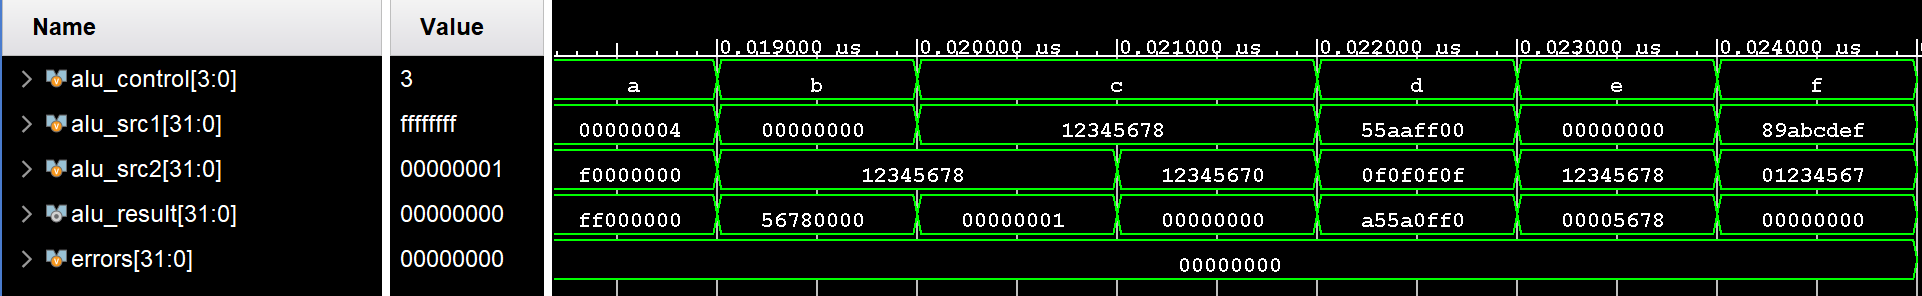
\includegraphics[width=\textwidth]{sim3.png}
    \caption{ALU仿真波形3}
\end{figure}

仿真脚本输出：
\begin{verbatim}
[PASS] ADD basic result=0x00000003
[PASS] ADD wrap result=0x00000000
[PASS] SUB basic result=0xfffffffe
[PASS] SLT -1<1 result=0x00000001
[PASS] SLT 5<-3 result=0x00000000
[PASS] SLTU 1<2 result=0x00000001
[PASS] SLTU FFFF<1 result=0x00000000
[PASS] AND result=0x050a0f00
[PASS] NOR result=0xa05000f0
[PASS] OR result=0x5fafff0f
[PASS] XOR result=0x5aa5f00f
[PASS] SLL by 4 result=0x00000110
[PASS] SRL by 4 result=0x0f000000
[PASS] SRA by 4 result=0xff000000
[PASS] LUI result=0x56780000
[PASS] SEQ equal result=0x00000001
[PASS] SEQ not equal result=0x00000000
[PASS] XNOR result=0xa55a0ff0
[PASS] LLI result=0x00005678
[PASS] RESERVED->0 result=0x00000000
\end{verbatim}

\subsection{上板验证}
\begin{enumerate}
    \item 拨码开关SW 0 1 2 3：四位控制编码从低位到高位；
    \item 拨码开关SW 6 ：输入选择，0 SRC1；1 SRC2；
\end{enumerate}

\begin{figure}[h]
    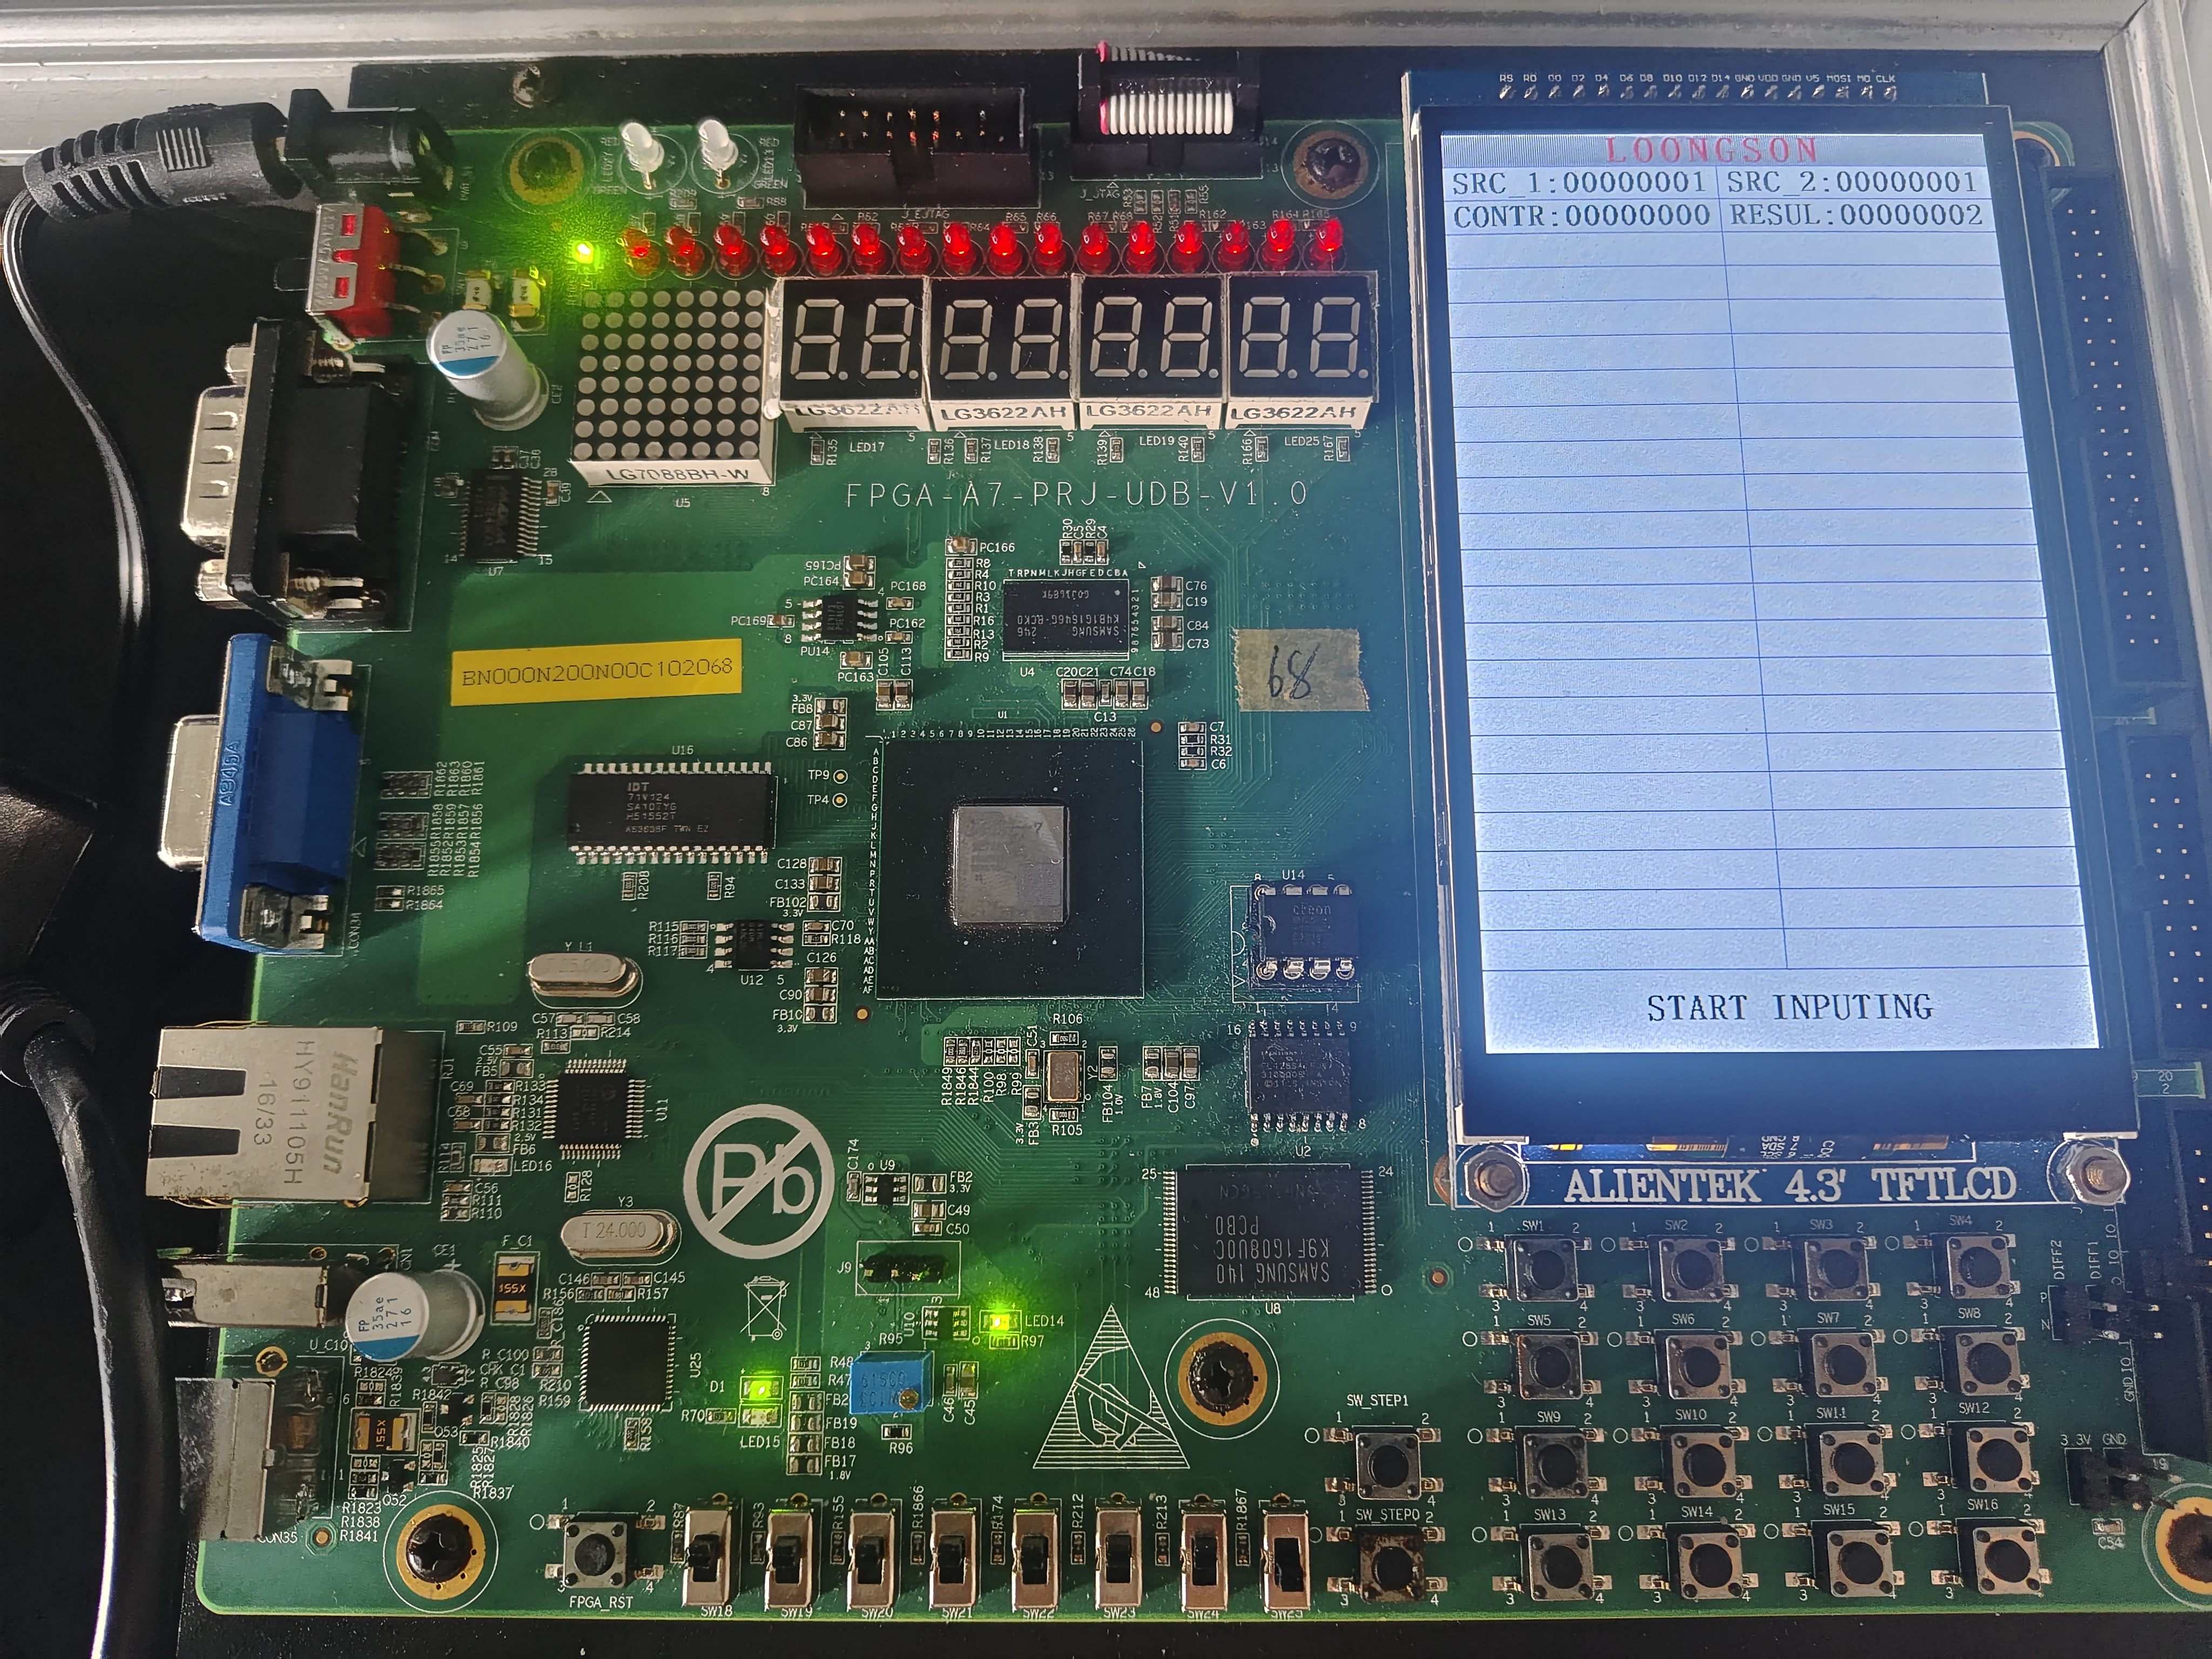
\includegraphics[width=\textwidth]{1.jpg}
    \caption{0000:ADD}
\end{figure}

\begin{figure}[h]
    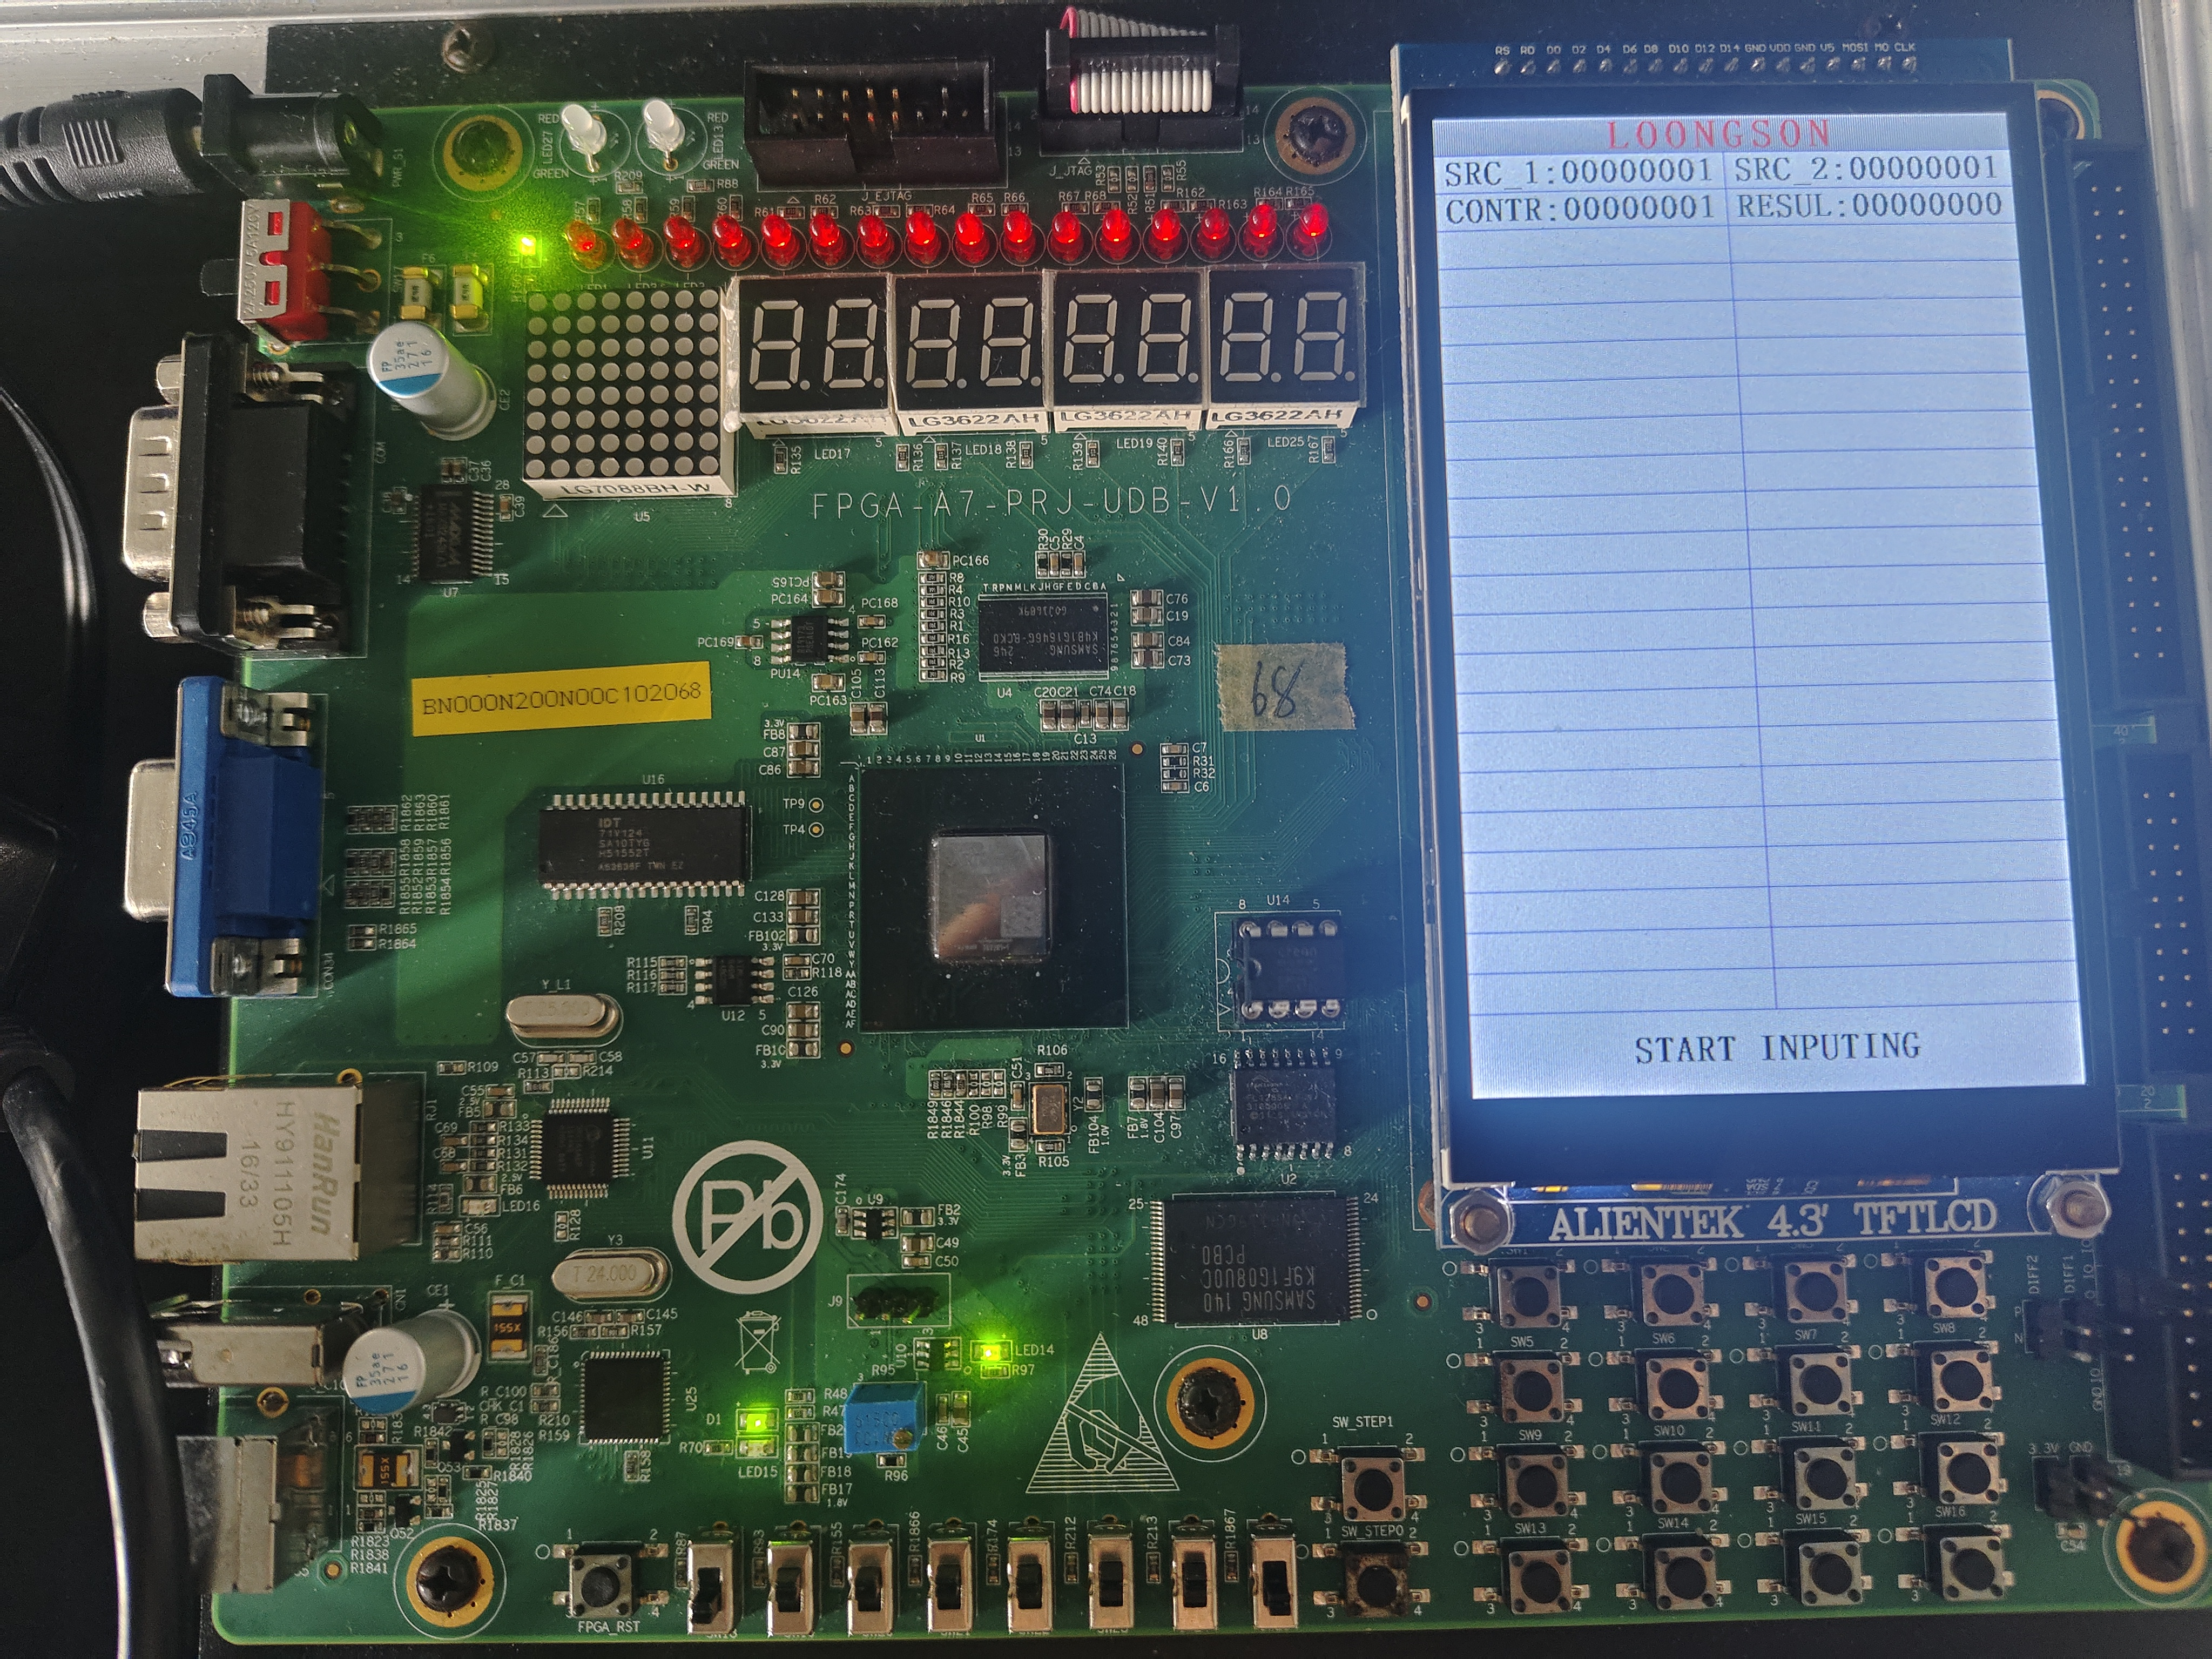
\includegraphics[width=\textwidth]{2.jpg}
    \caption{0001:SUB}
\end{figure}

\begin{figure}[h]
    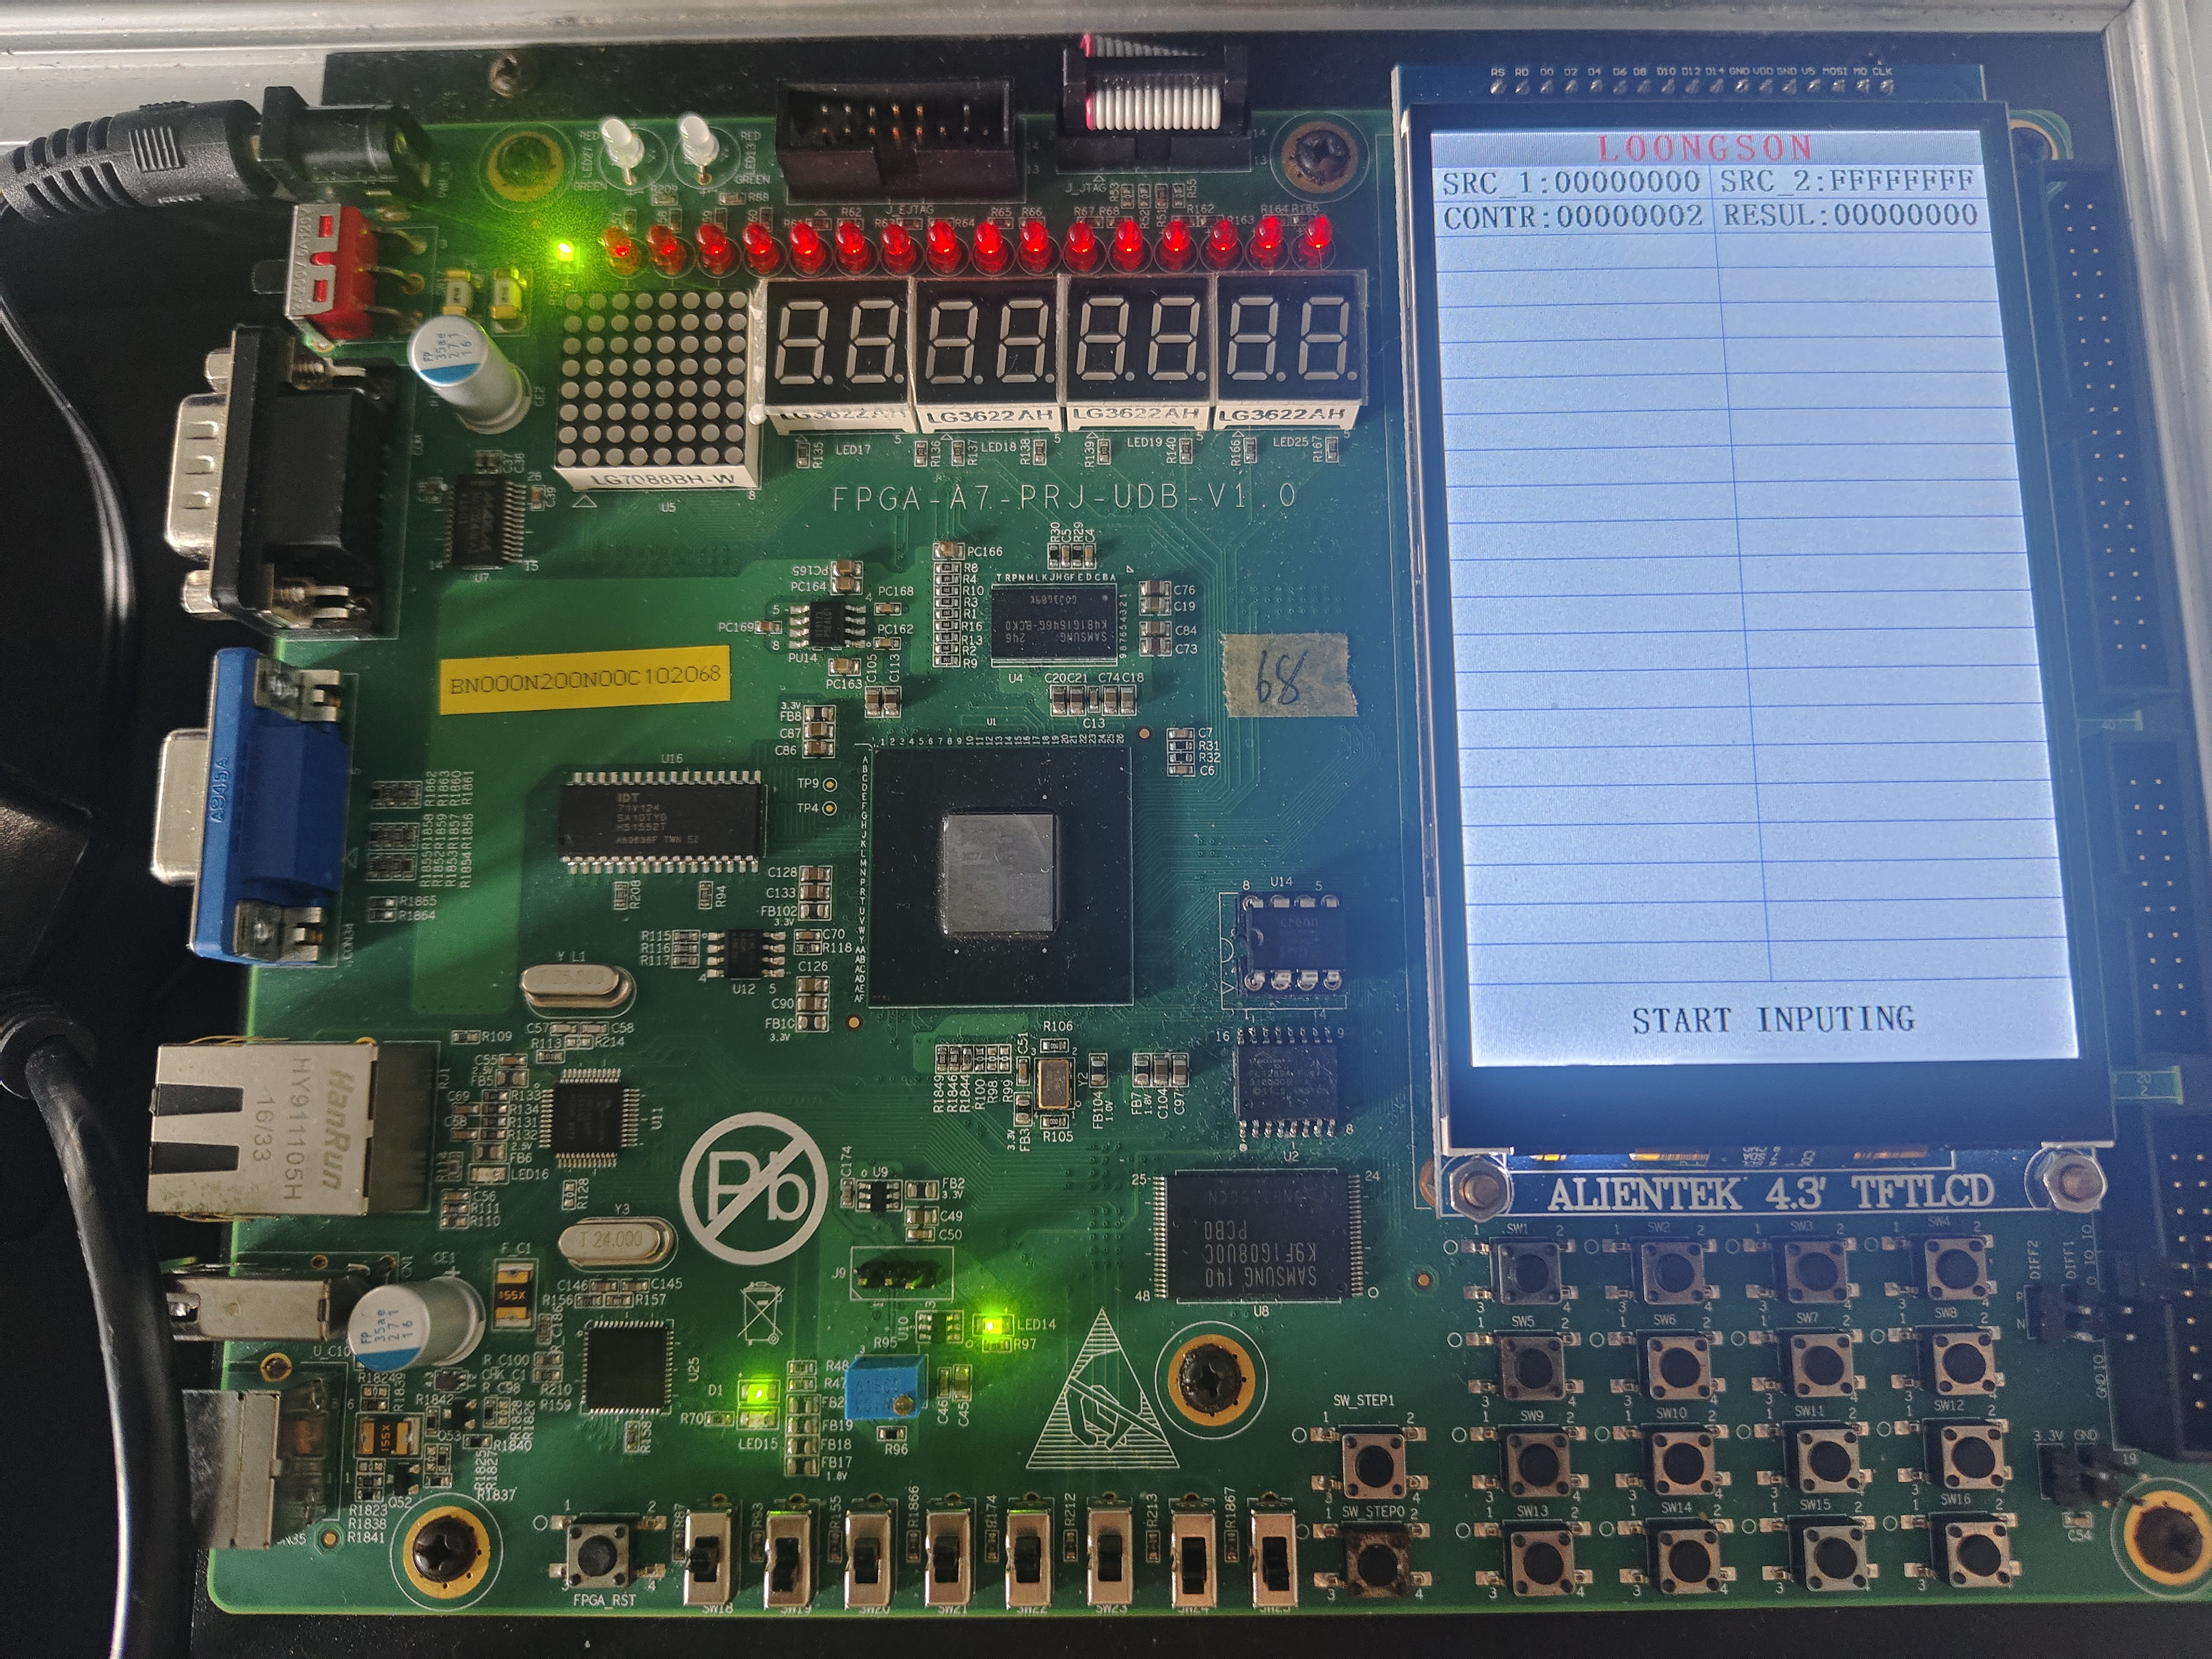
\includegraphics[width=\textwidth]{3.jpg}
    \caption{0010:SLT}
\end{figure}

\begin{figure}[h]
    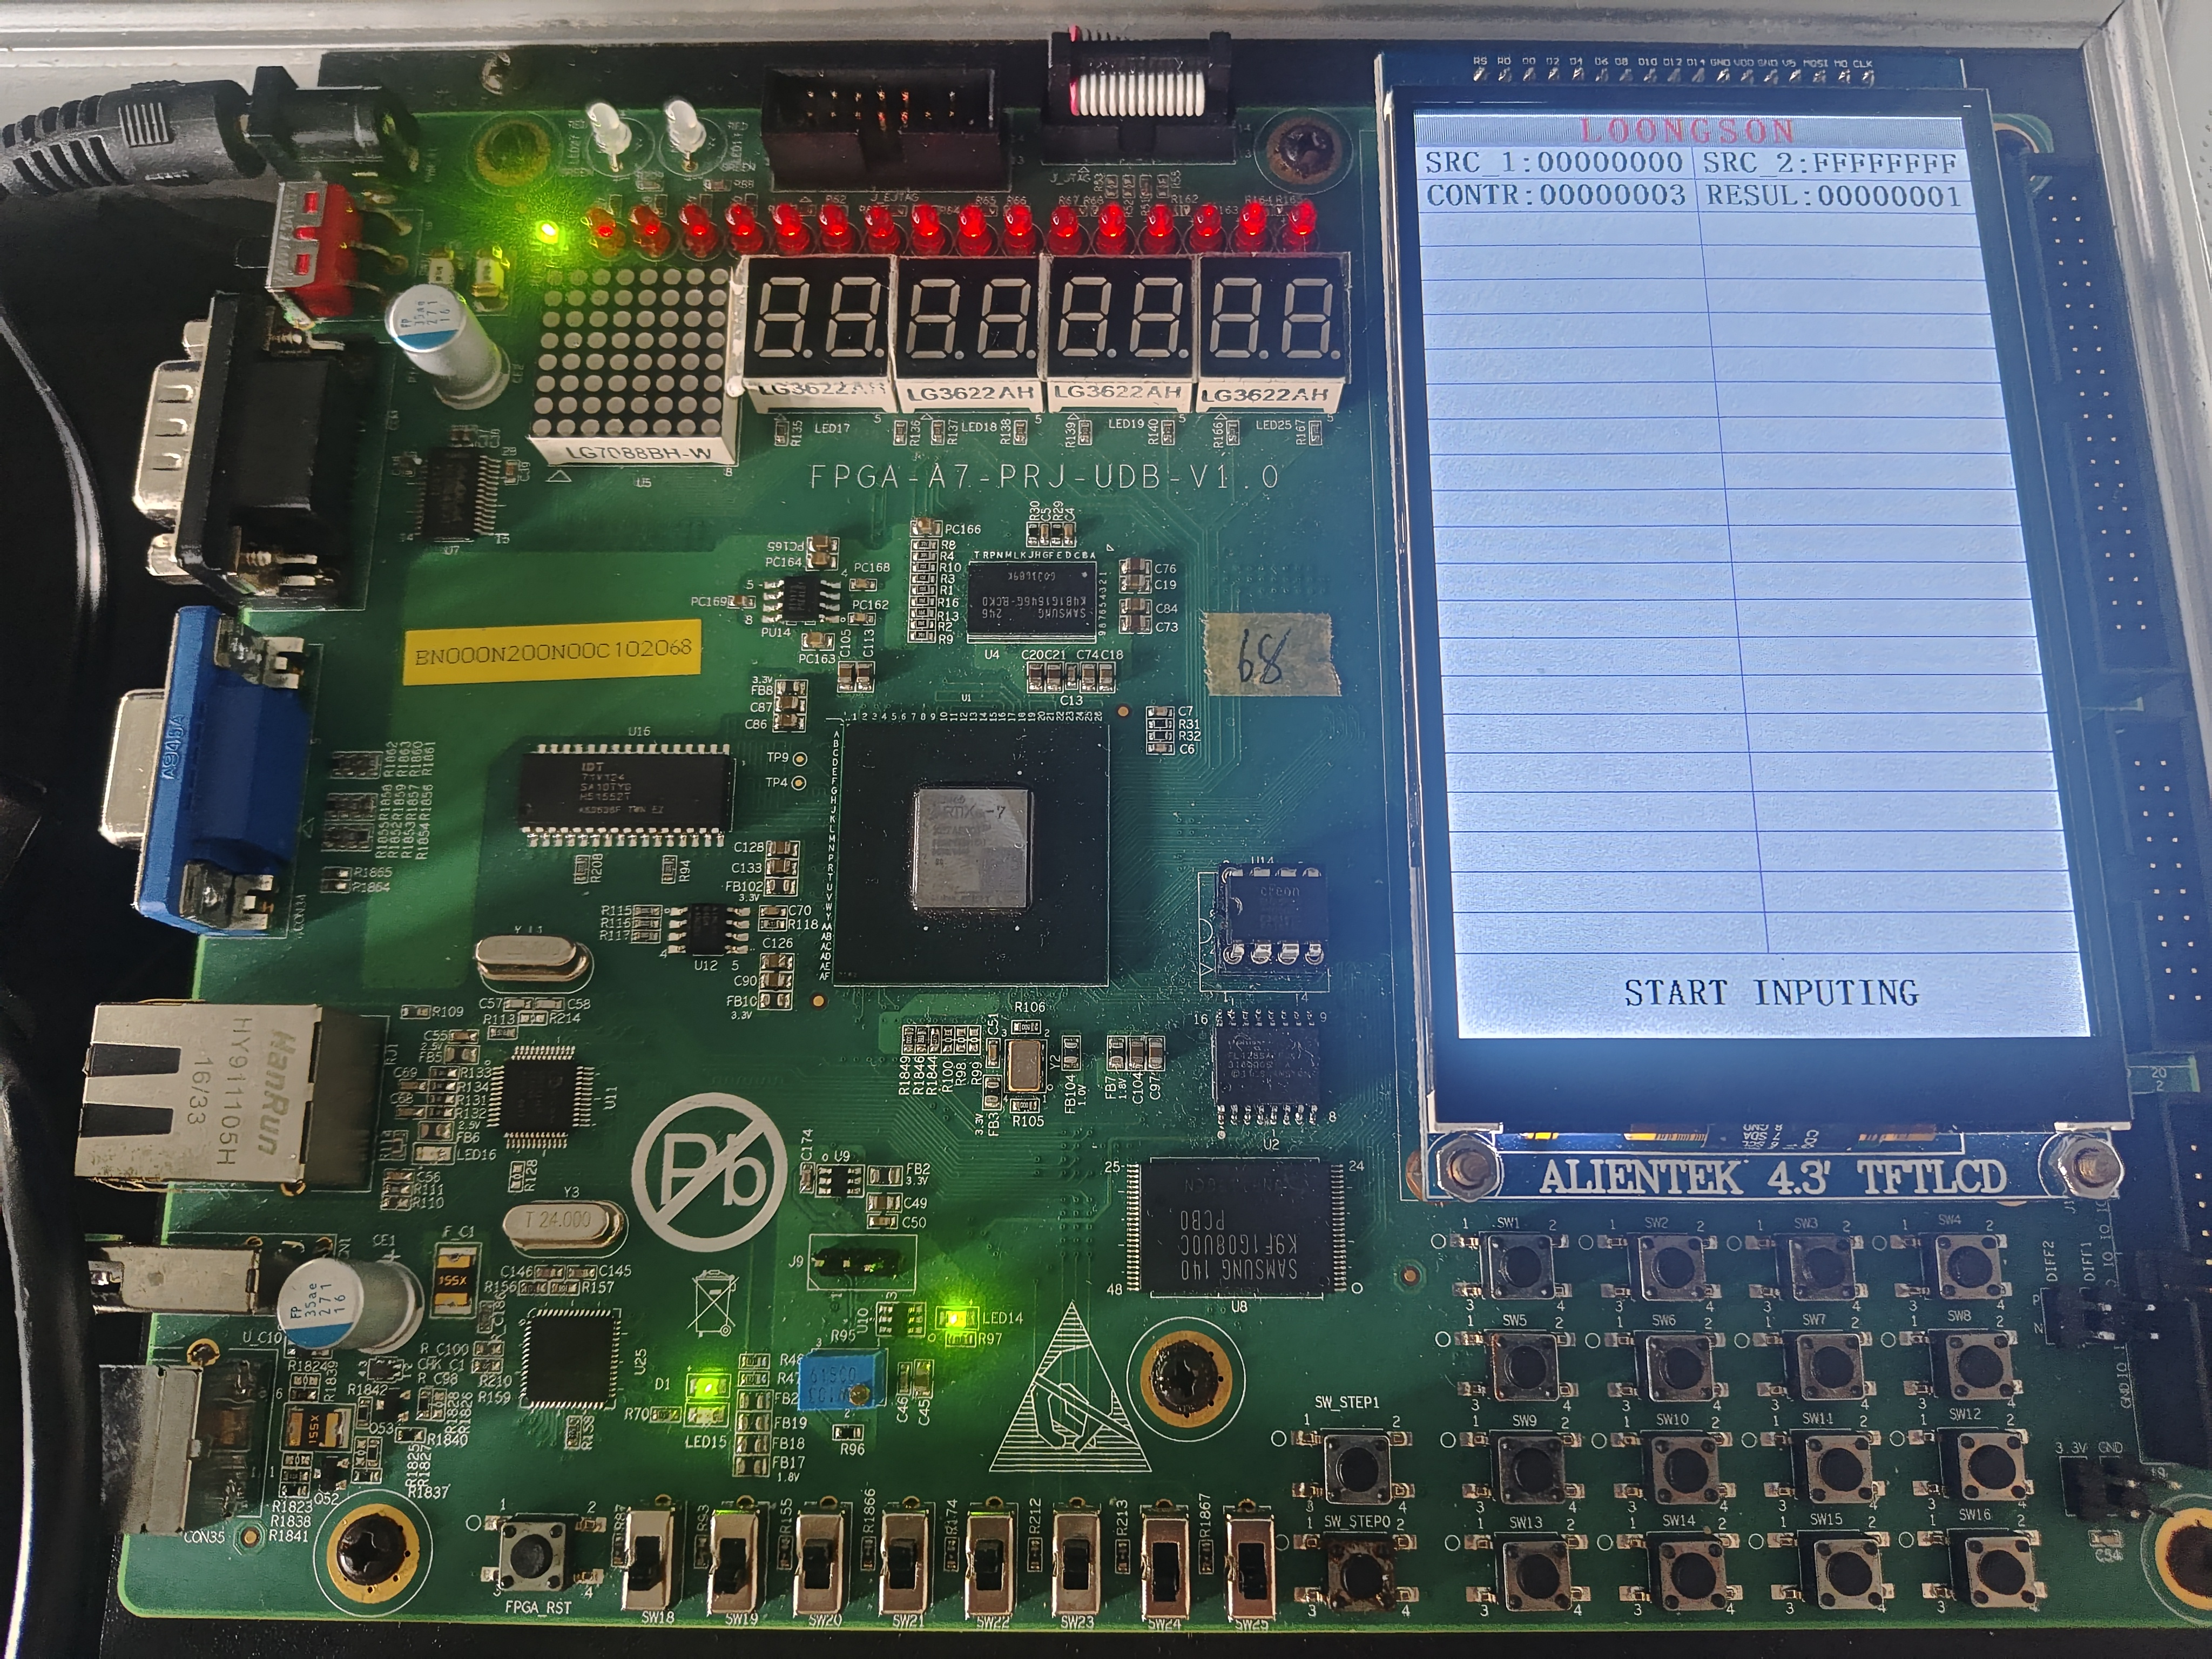
\includegraphics[width=\textwidth]{4.jpg}
    \caption{0011:SLTU}
\end{figure}

\begin{figure}[!h]
    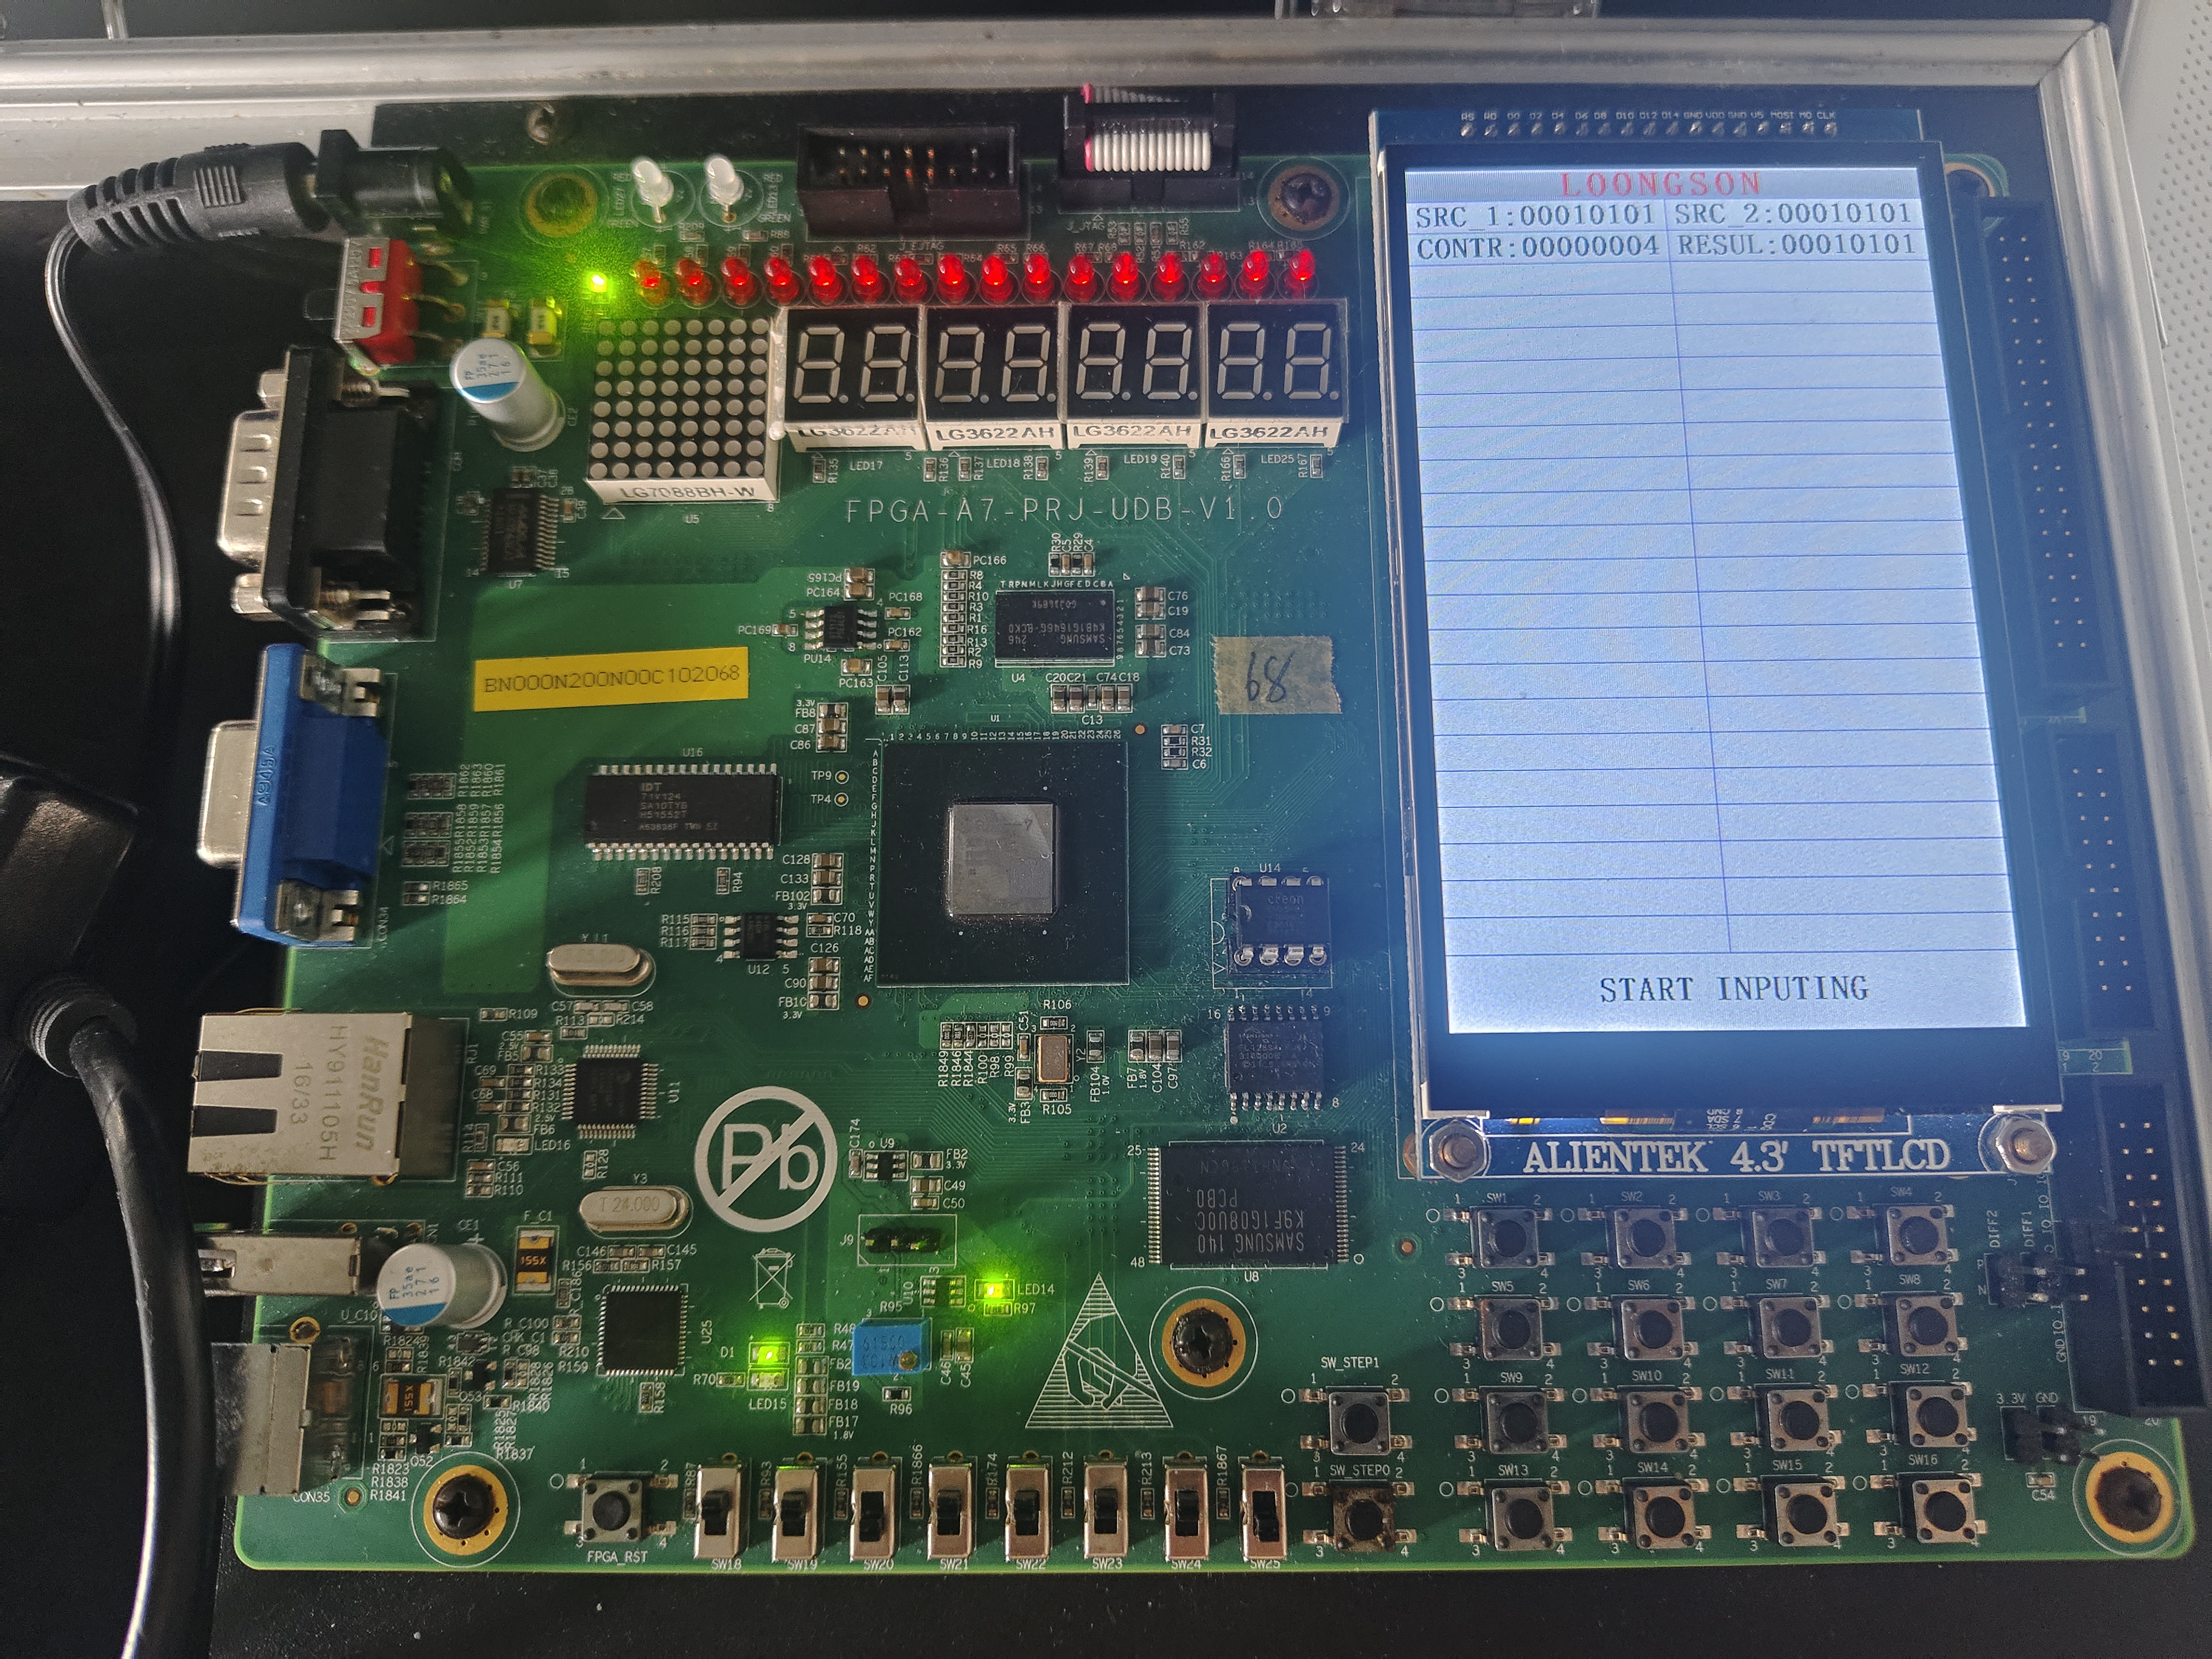
\includegraphics[width=\textwidth]{5.jpg}
    \caption{0100:AND}
\end{figure}

\begin{figure}[!h]
    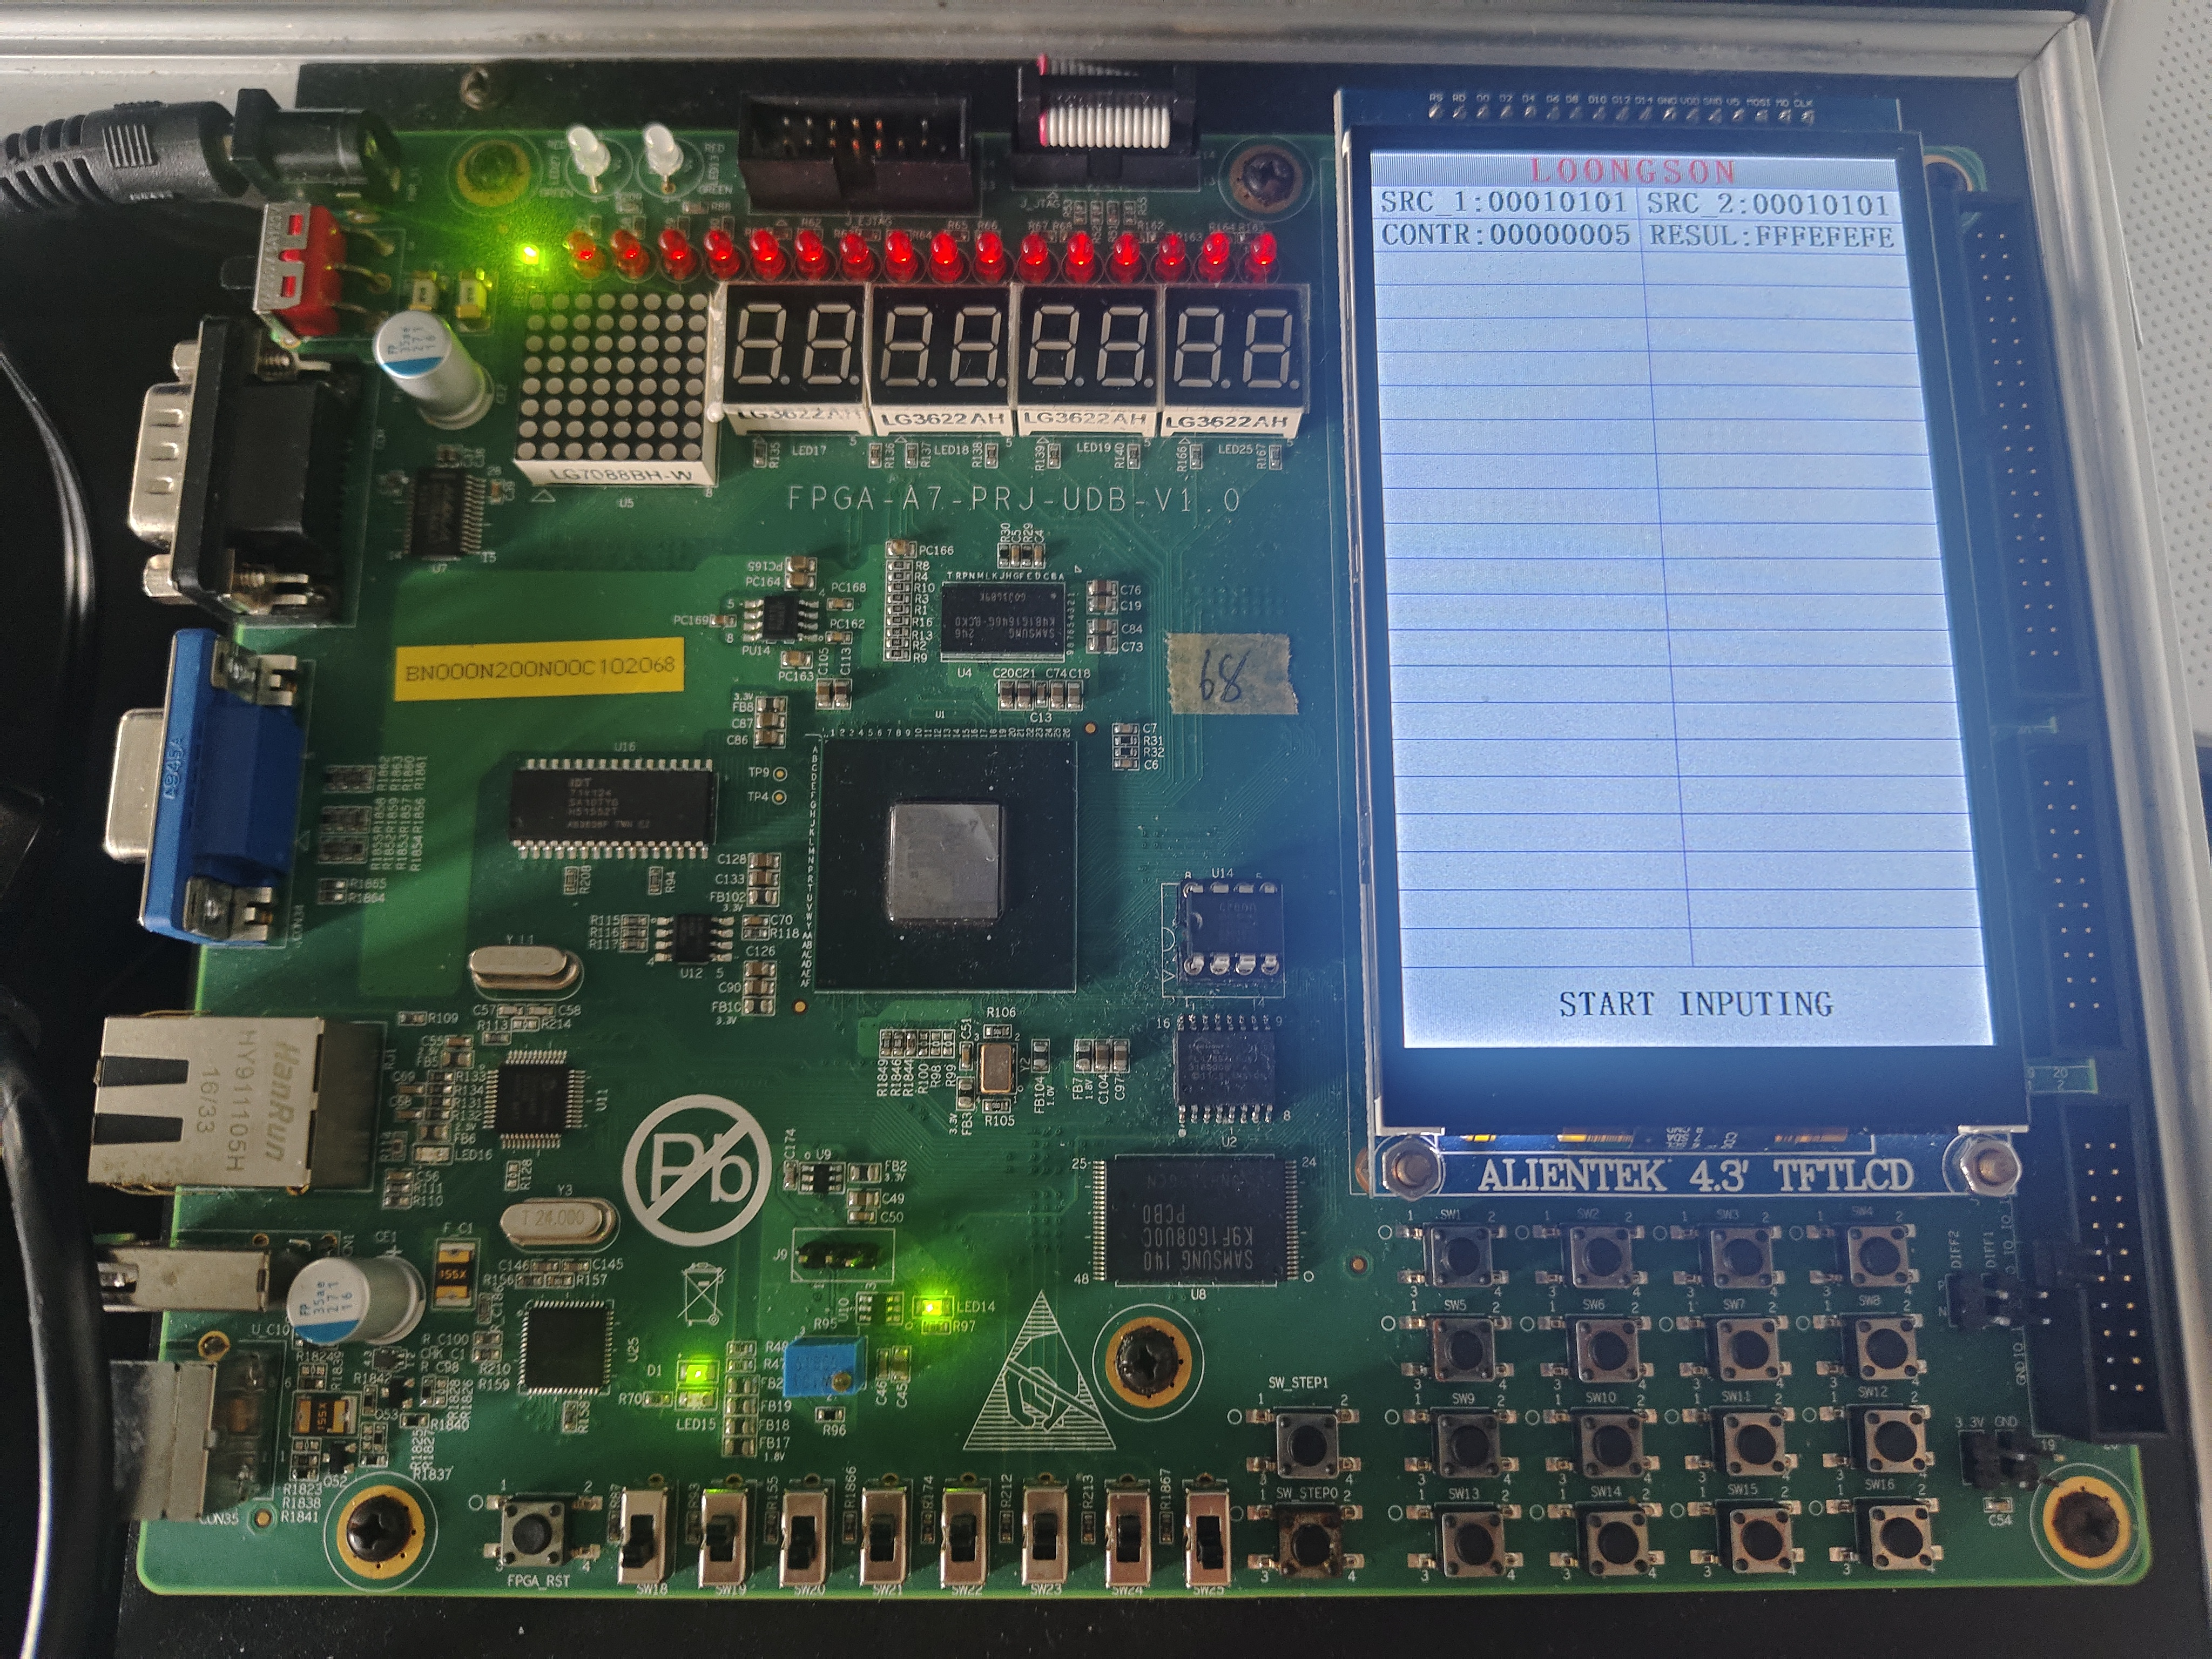
\includegraphics[width=\textwidth]{6.jpg}
    \caption{0101:NOR}
\end{figure}

\begin{figure}[h]
    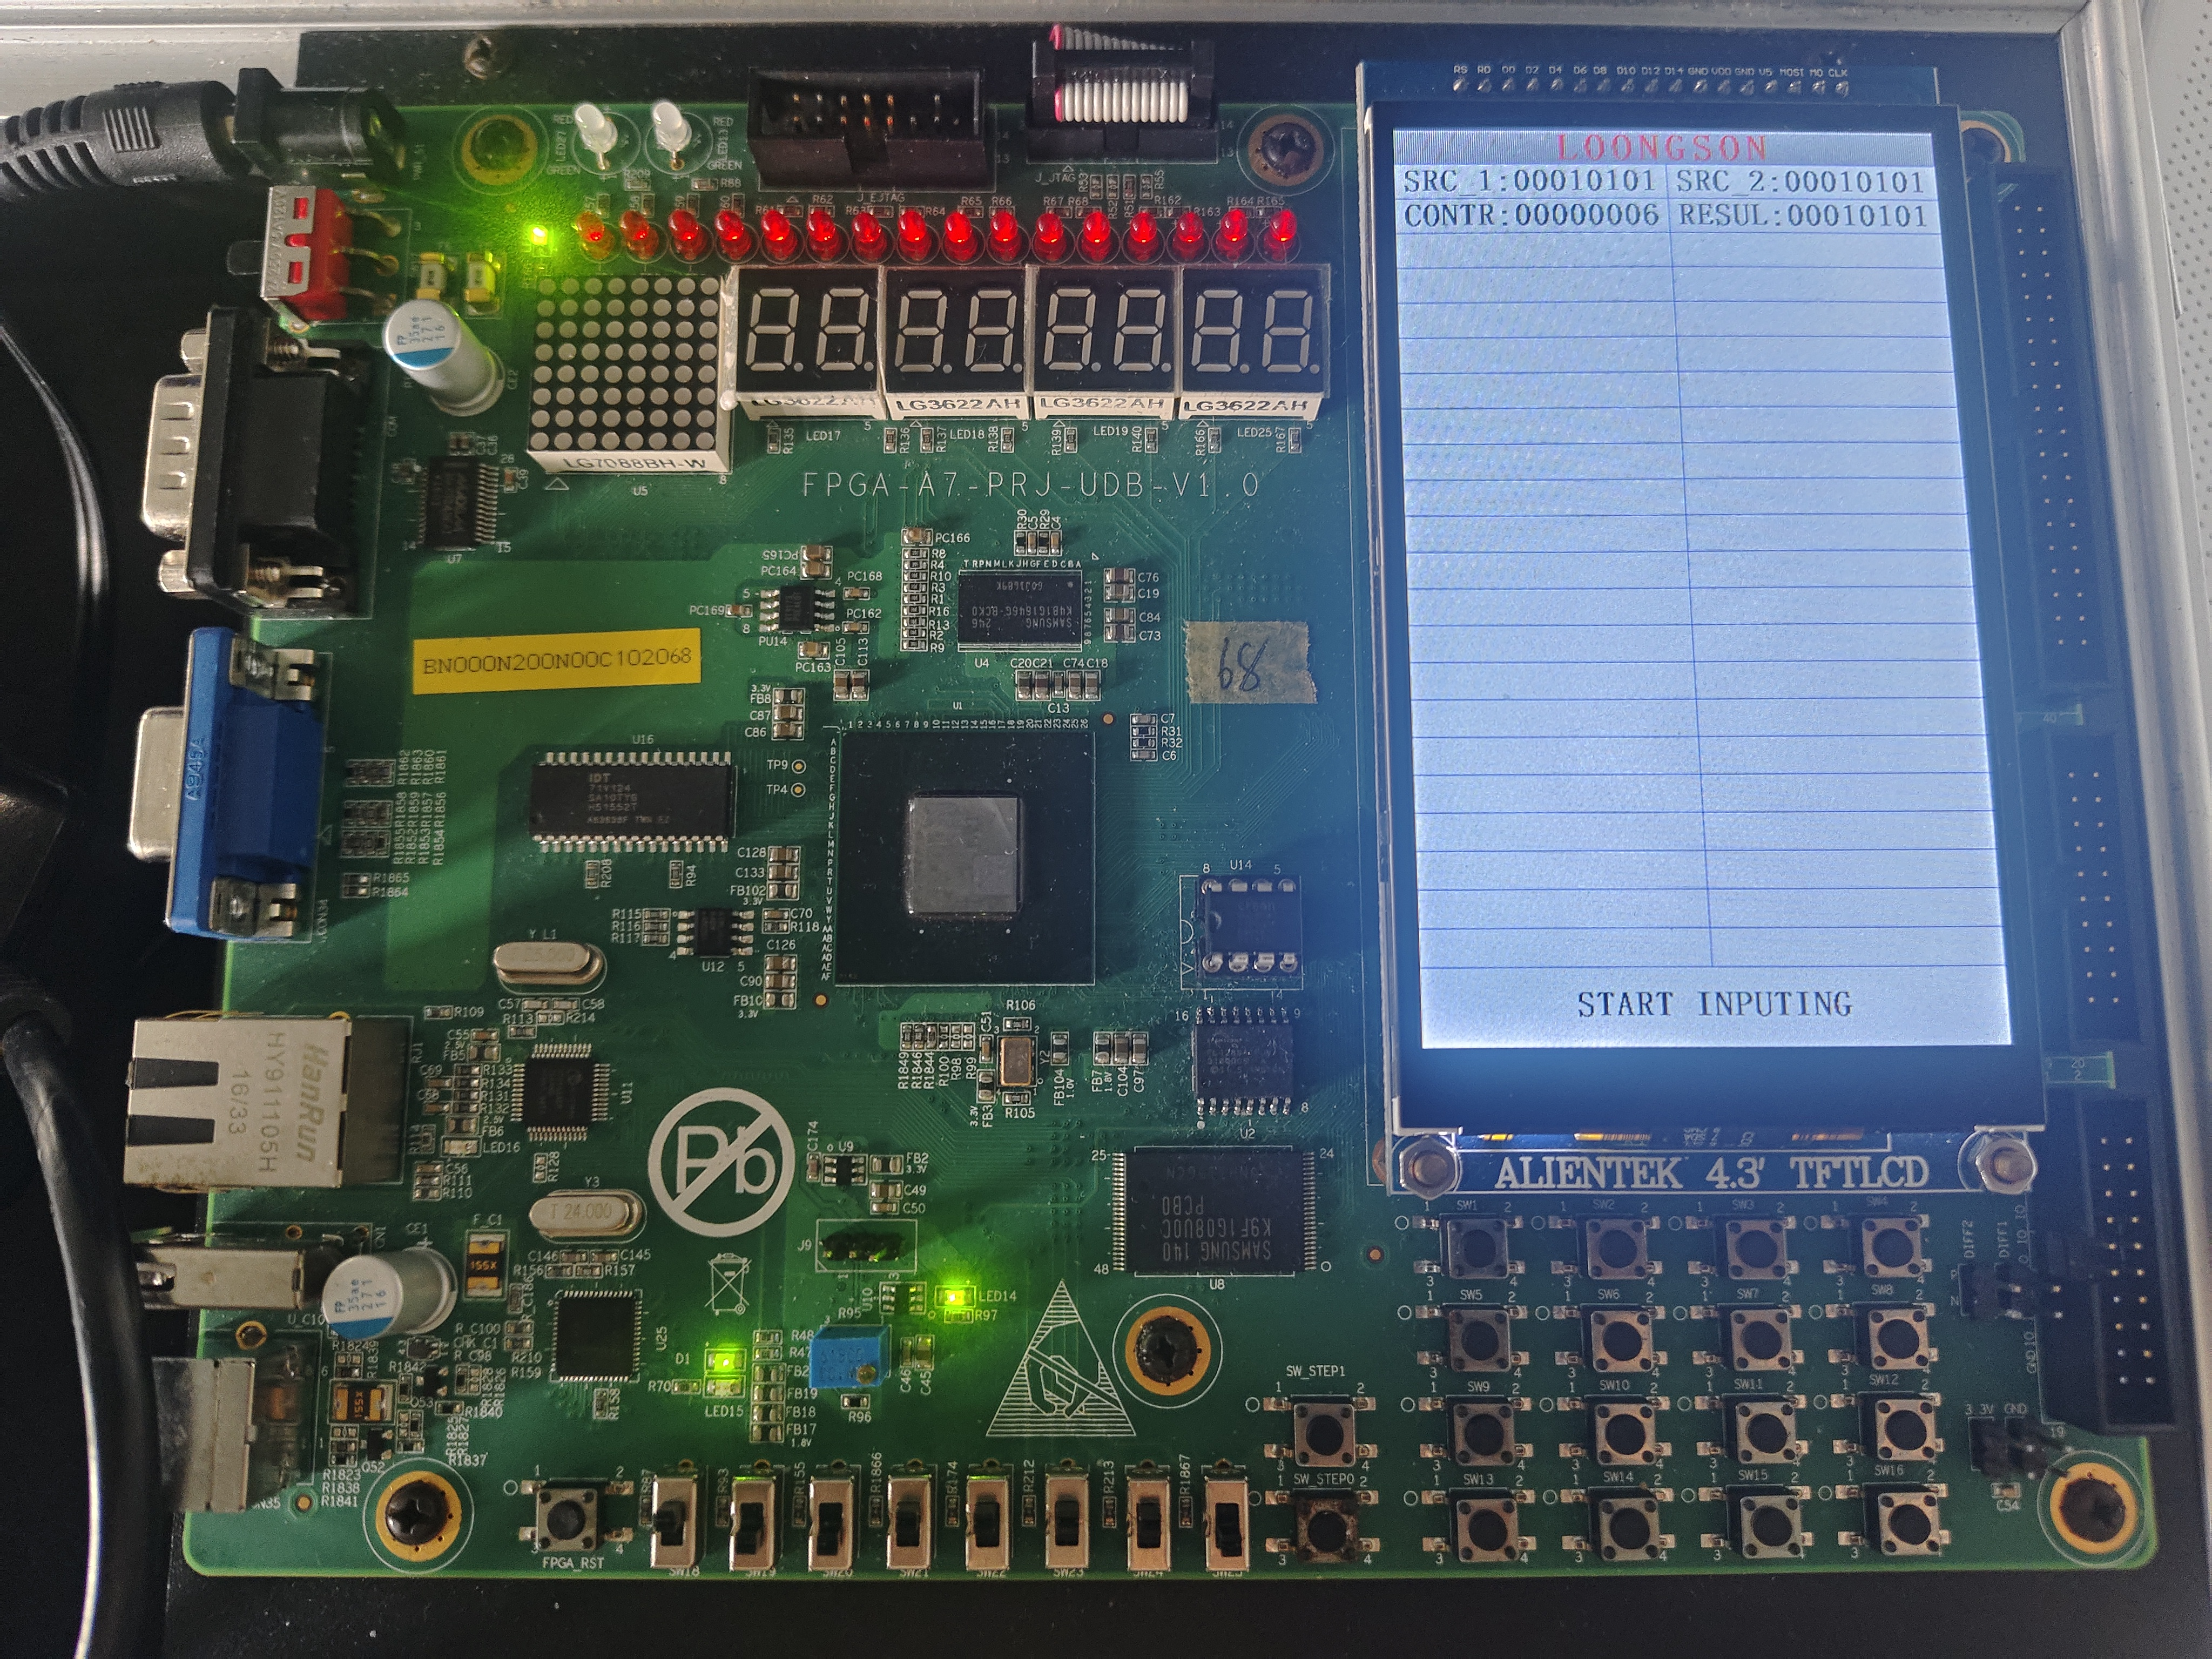
\includegraphics[width=\textwidth]{7.jpg}
    \caption{0110:OR}
\end{figure}

\begin{figure}[h]
    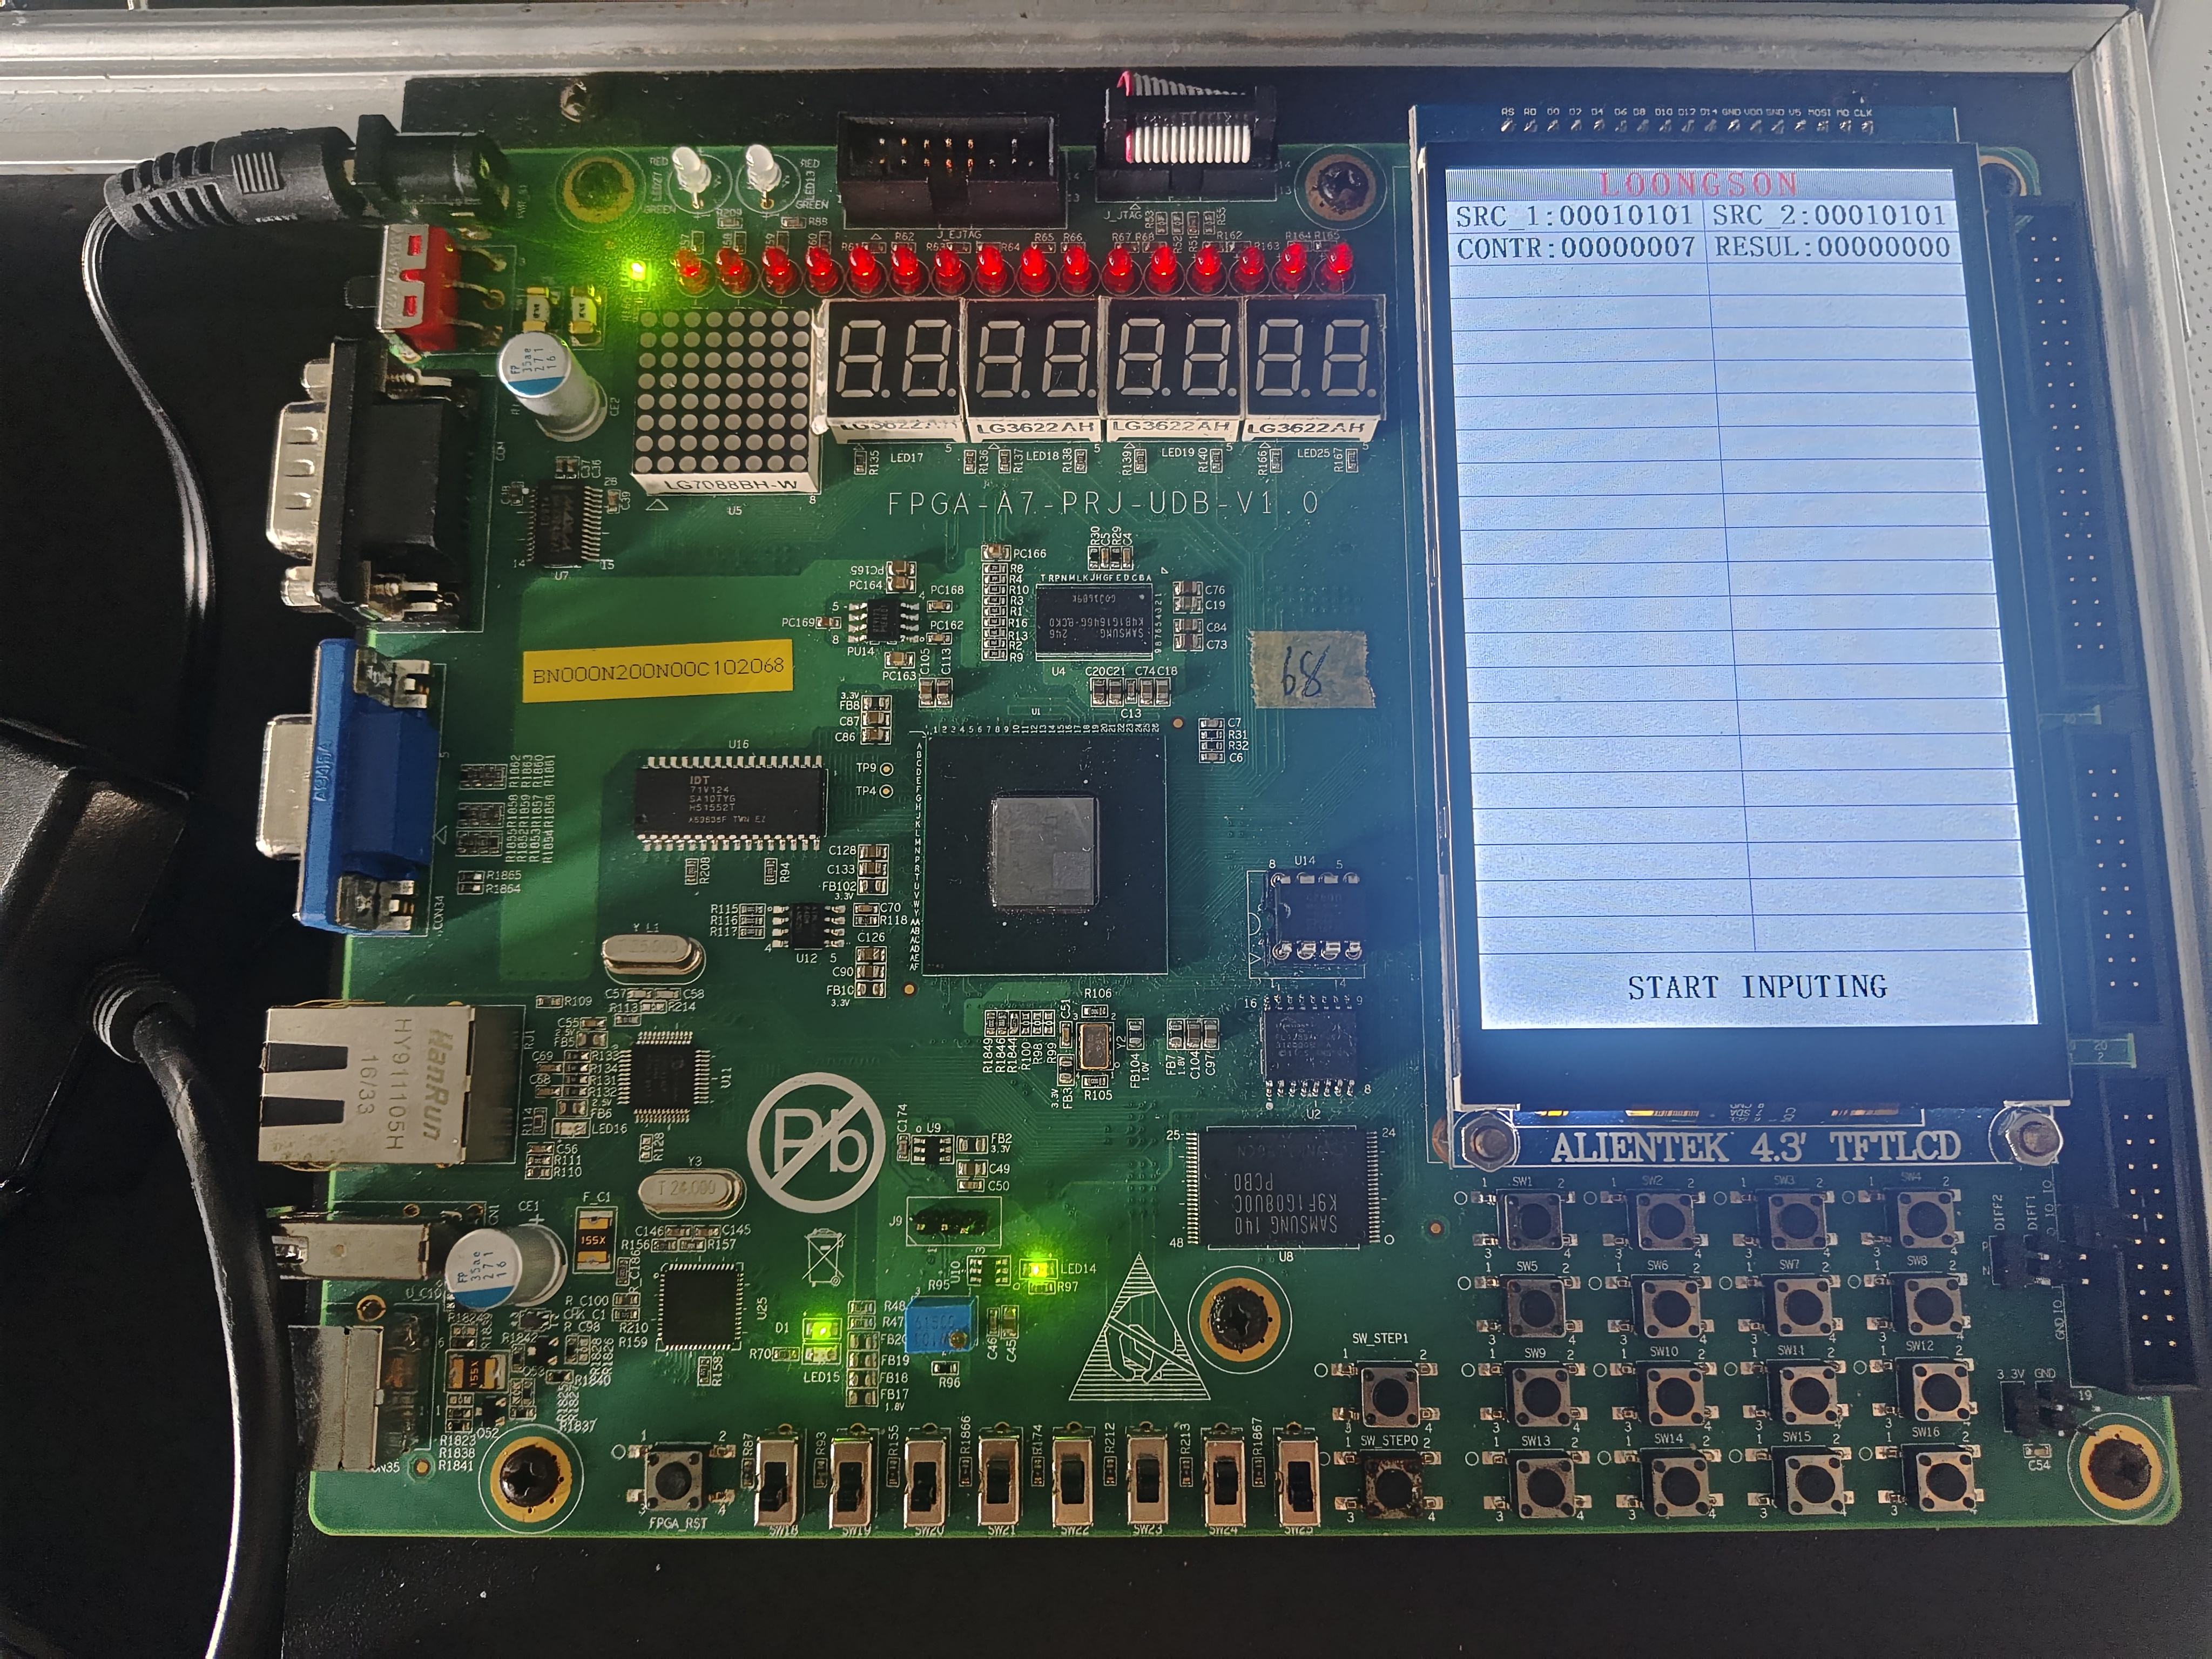
\includegraphics[width=\textwidth]{8.jpg}
    \caption{0111:XOR}
\end{figure}

\begin{figure}[h]
    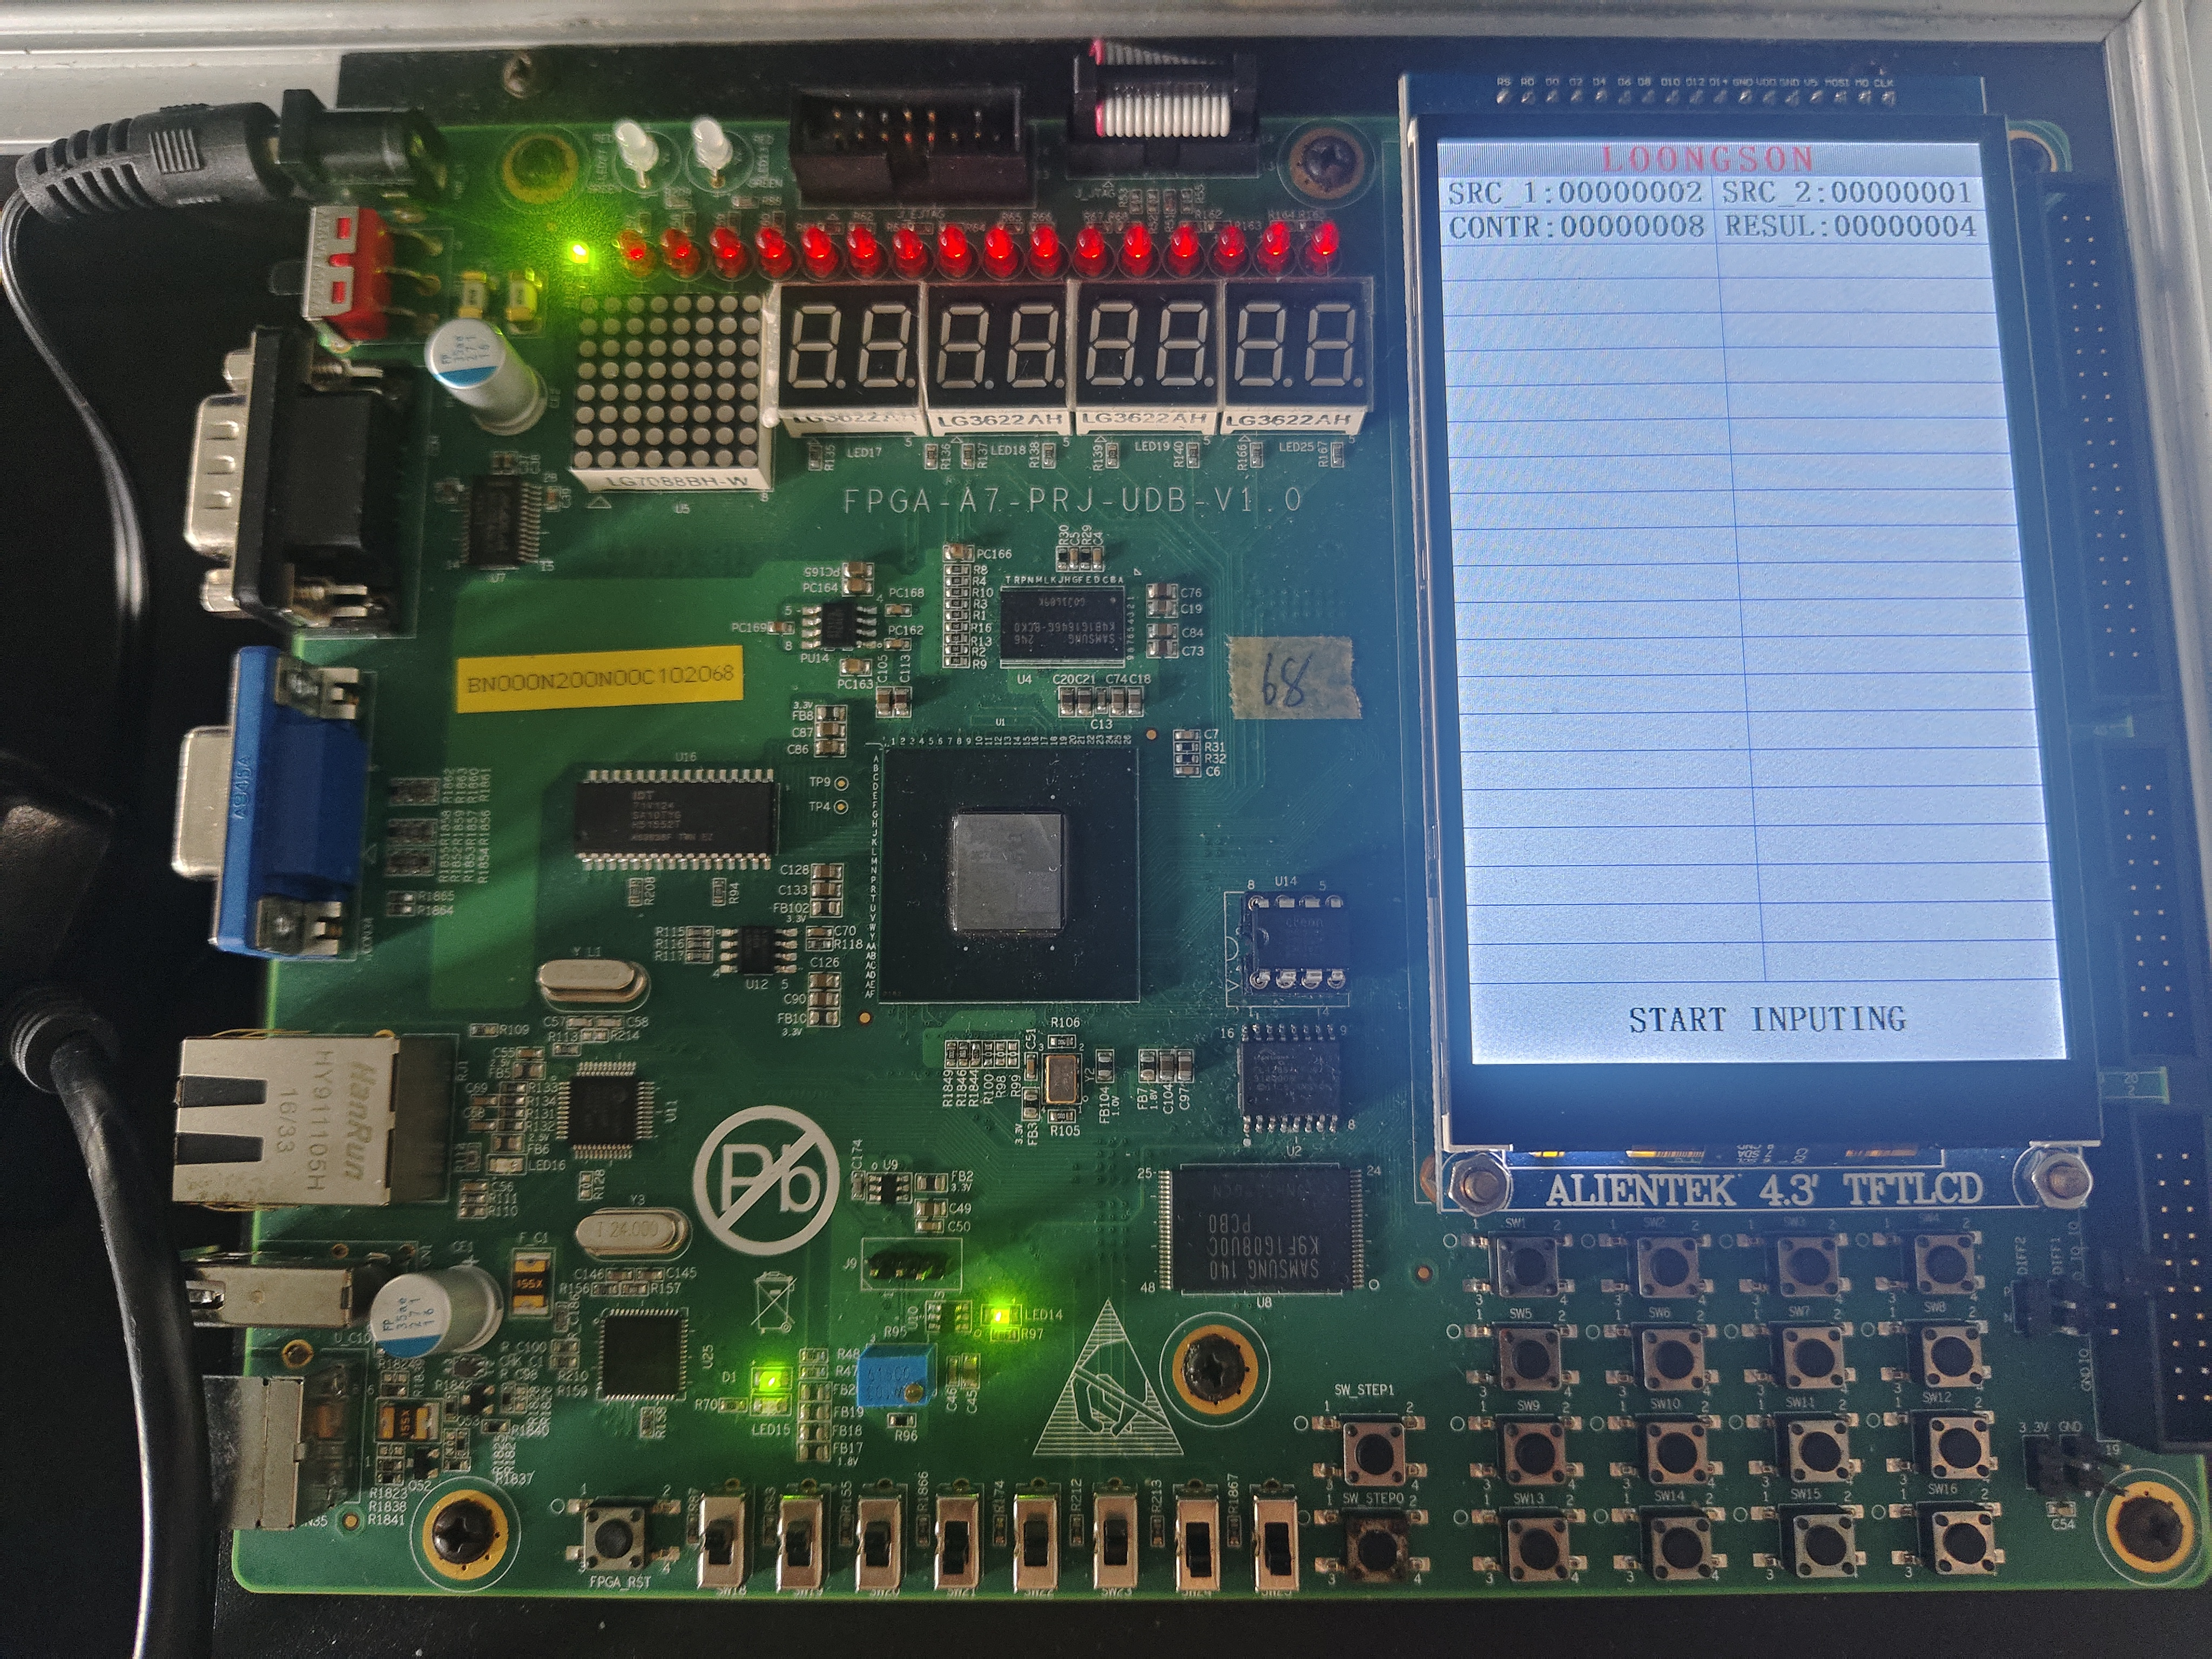
\includegraphics[width=\textwidth]{9.jpg}
    \caption{1000:SLL}
\end{figure}

\begin{figure}[h]
    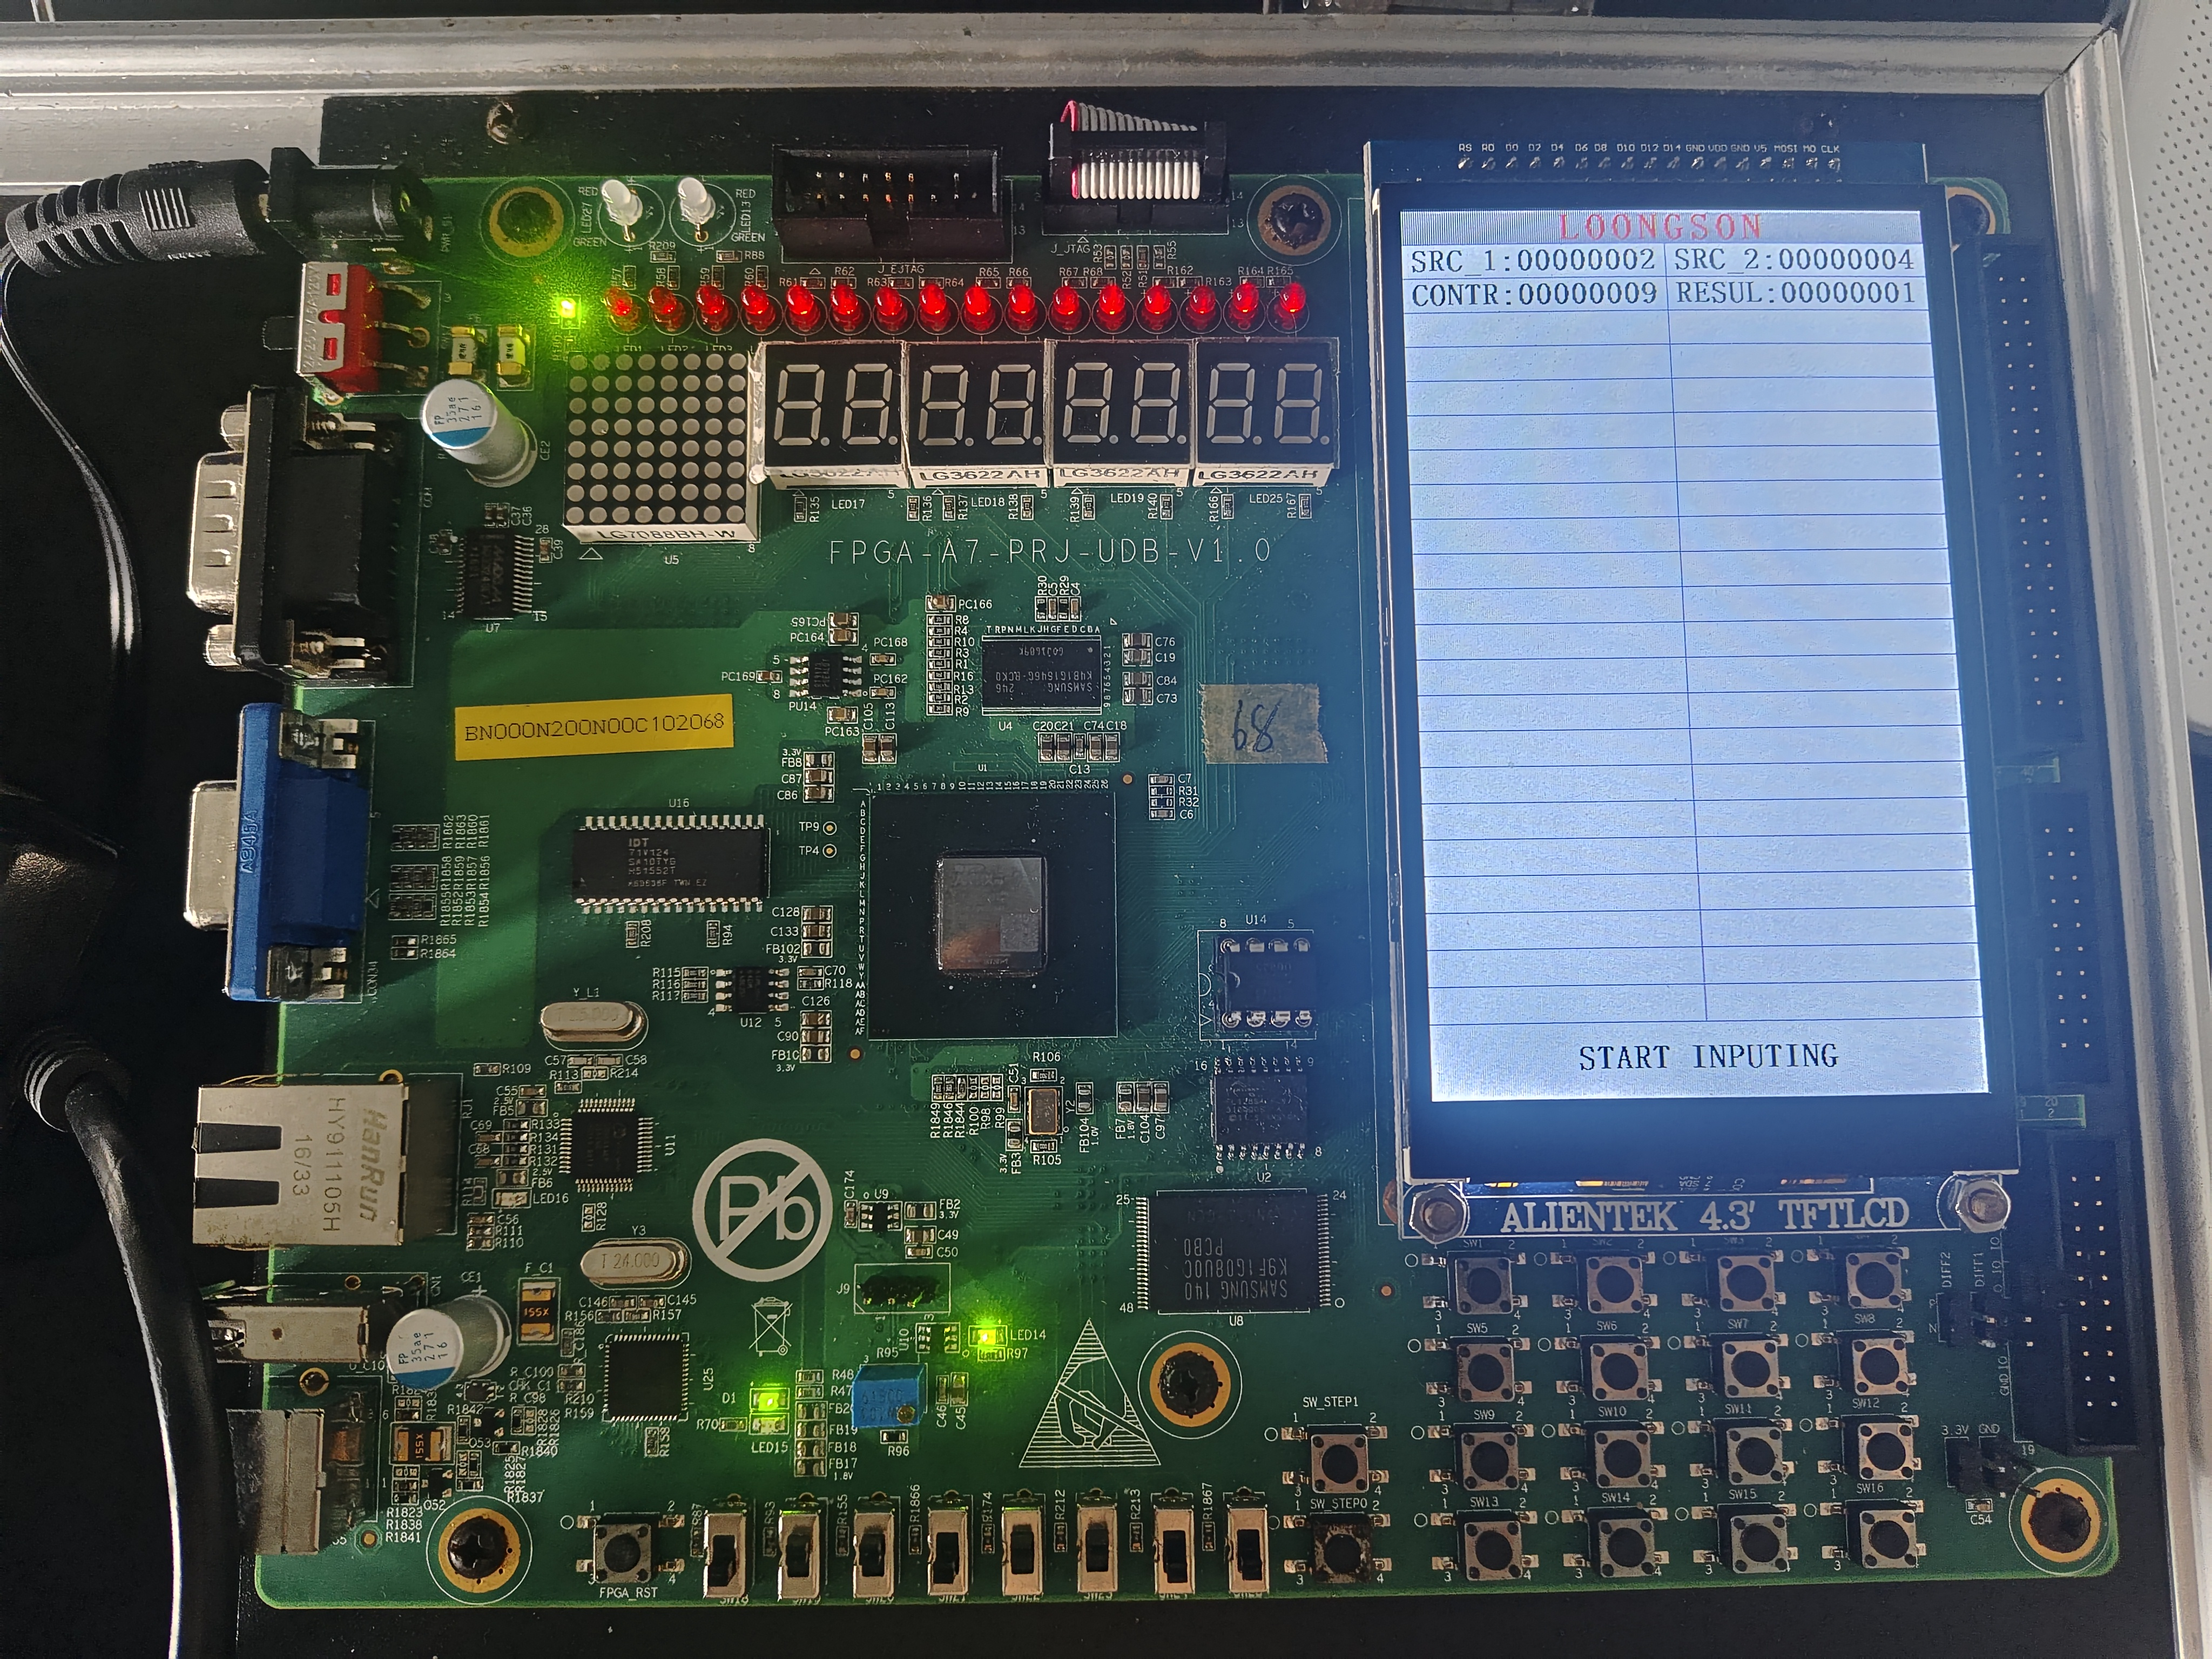
\includegraphics[width=\textwidth]{10.jpg}
    \caption{1001:SRL}
\end{figure}

\begin{figure}[h]
    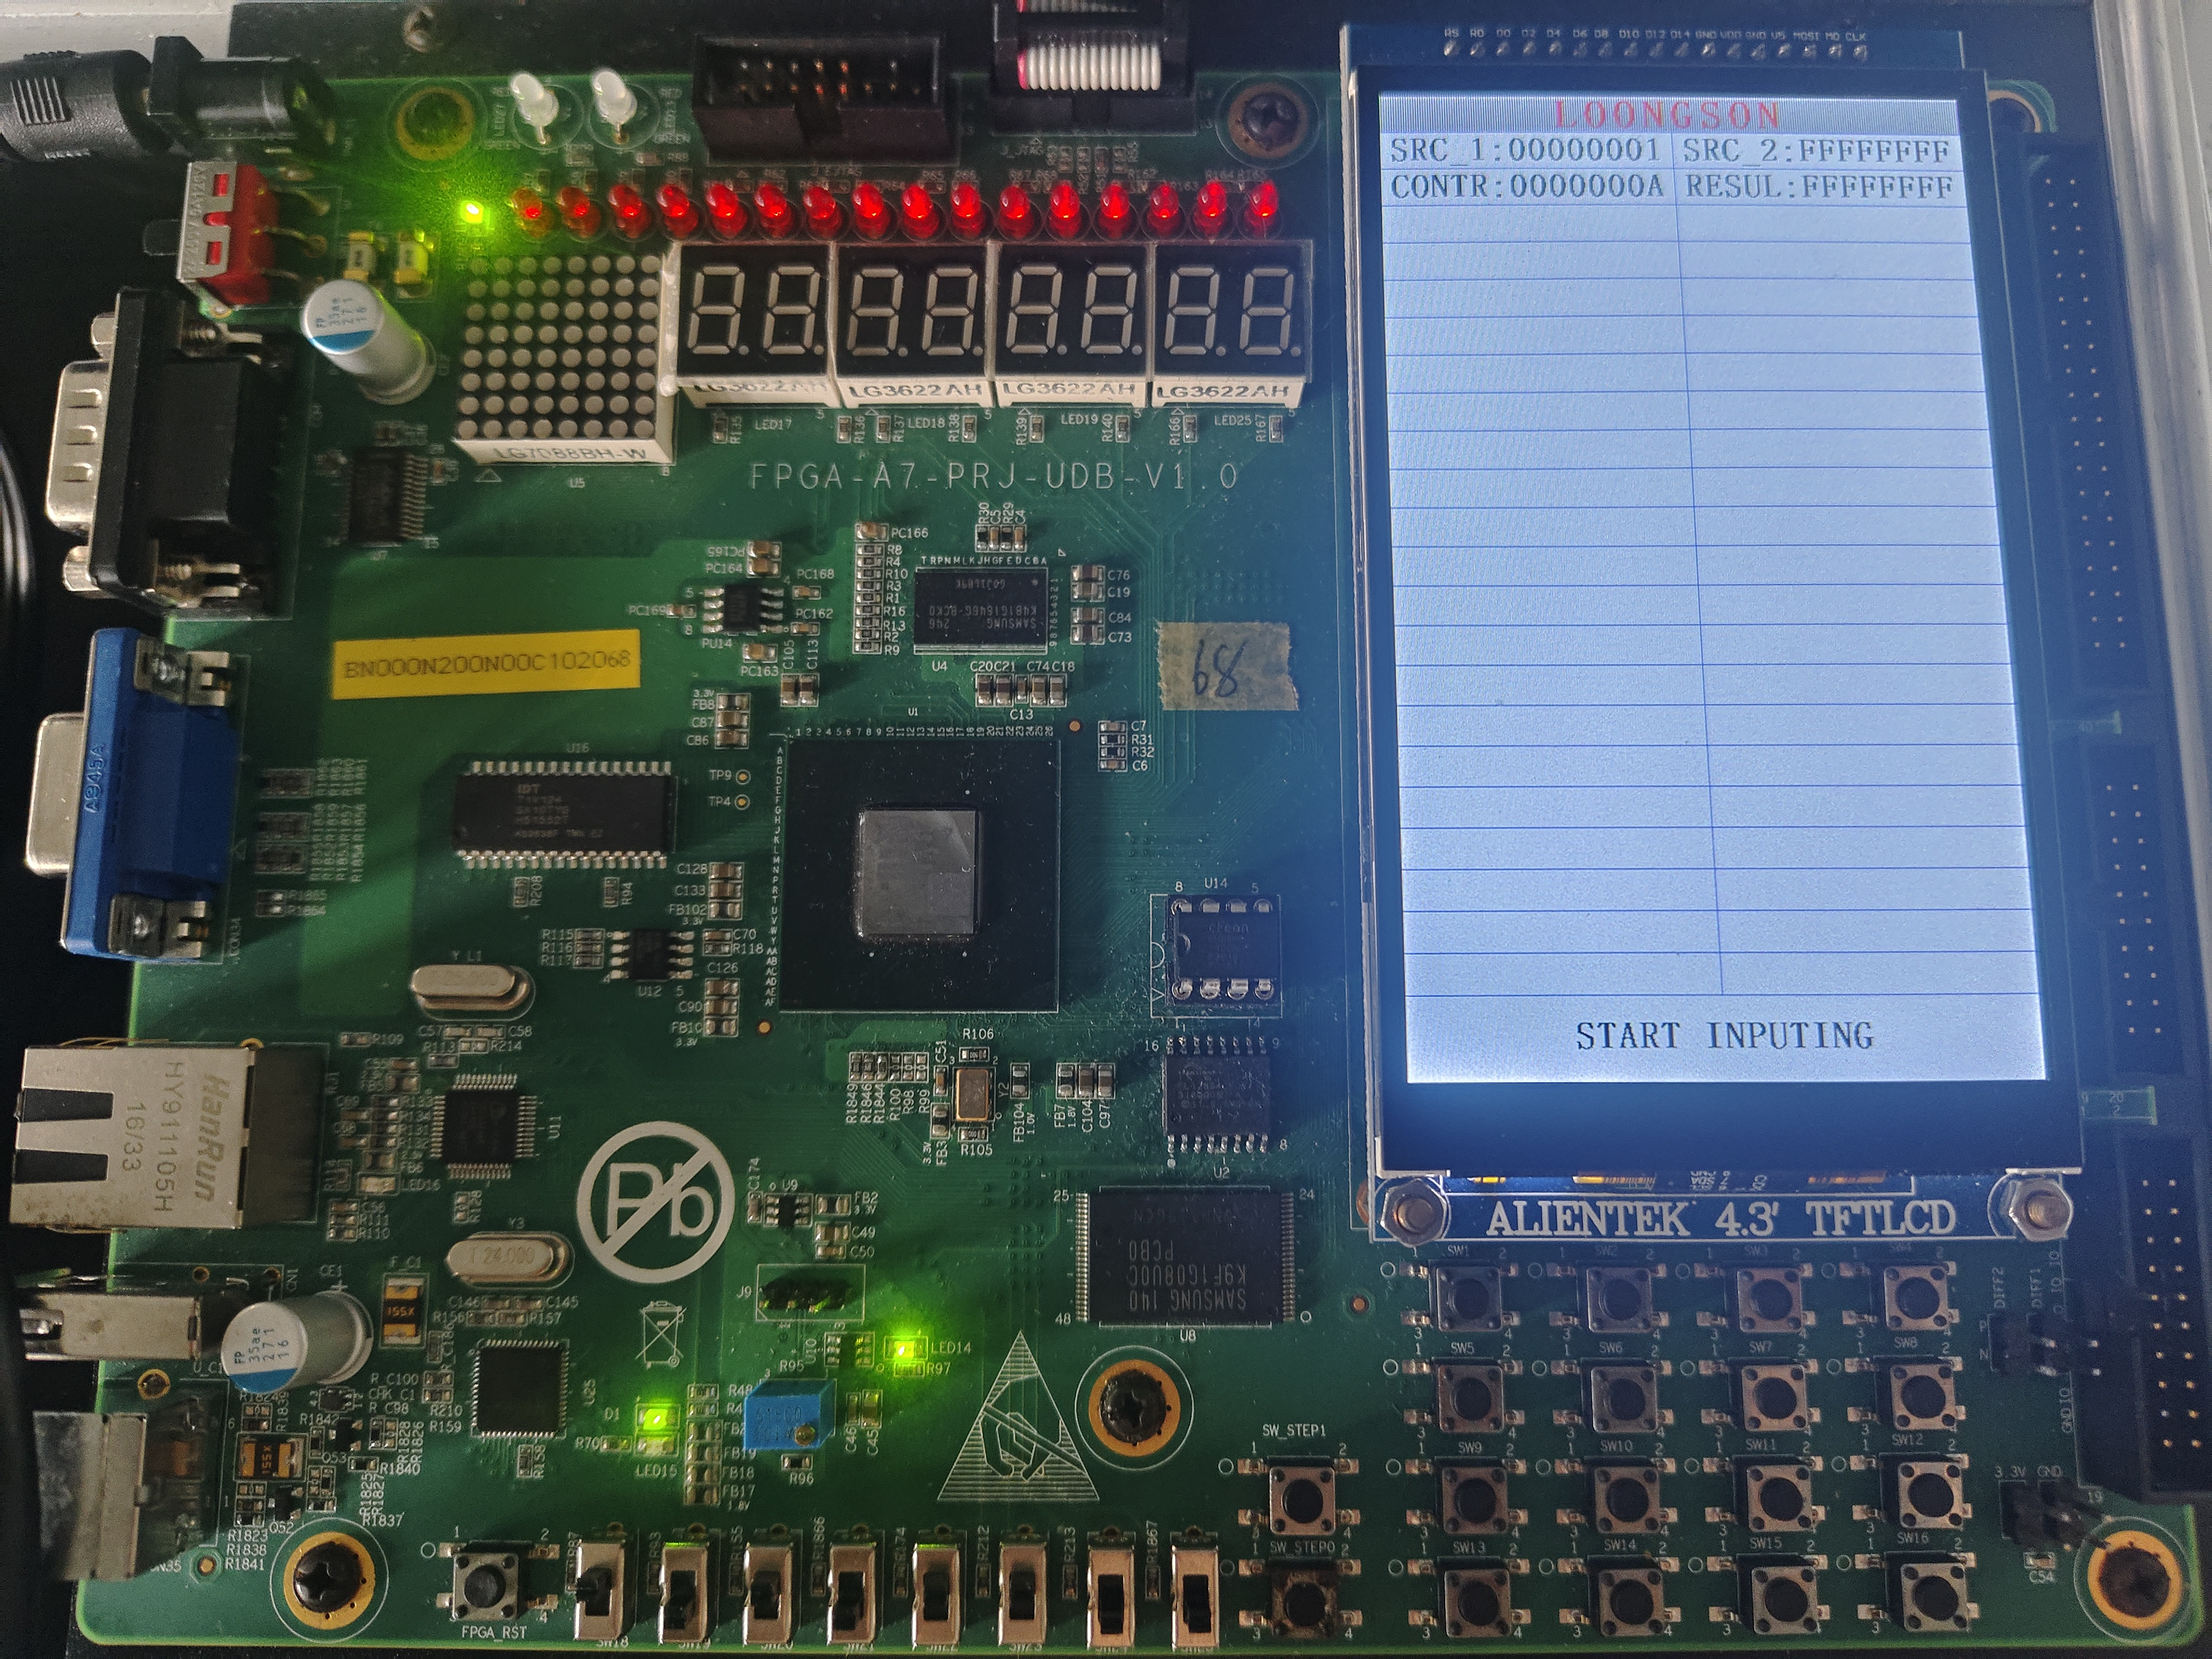
\includegraphics[width=\textwidth]{11.jpg}
    \caption{1010:SRA}
\end{figure}

\begin{figure}[h]
    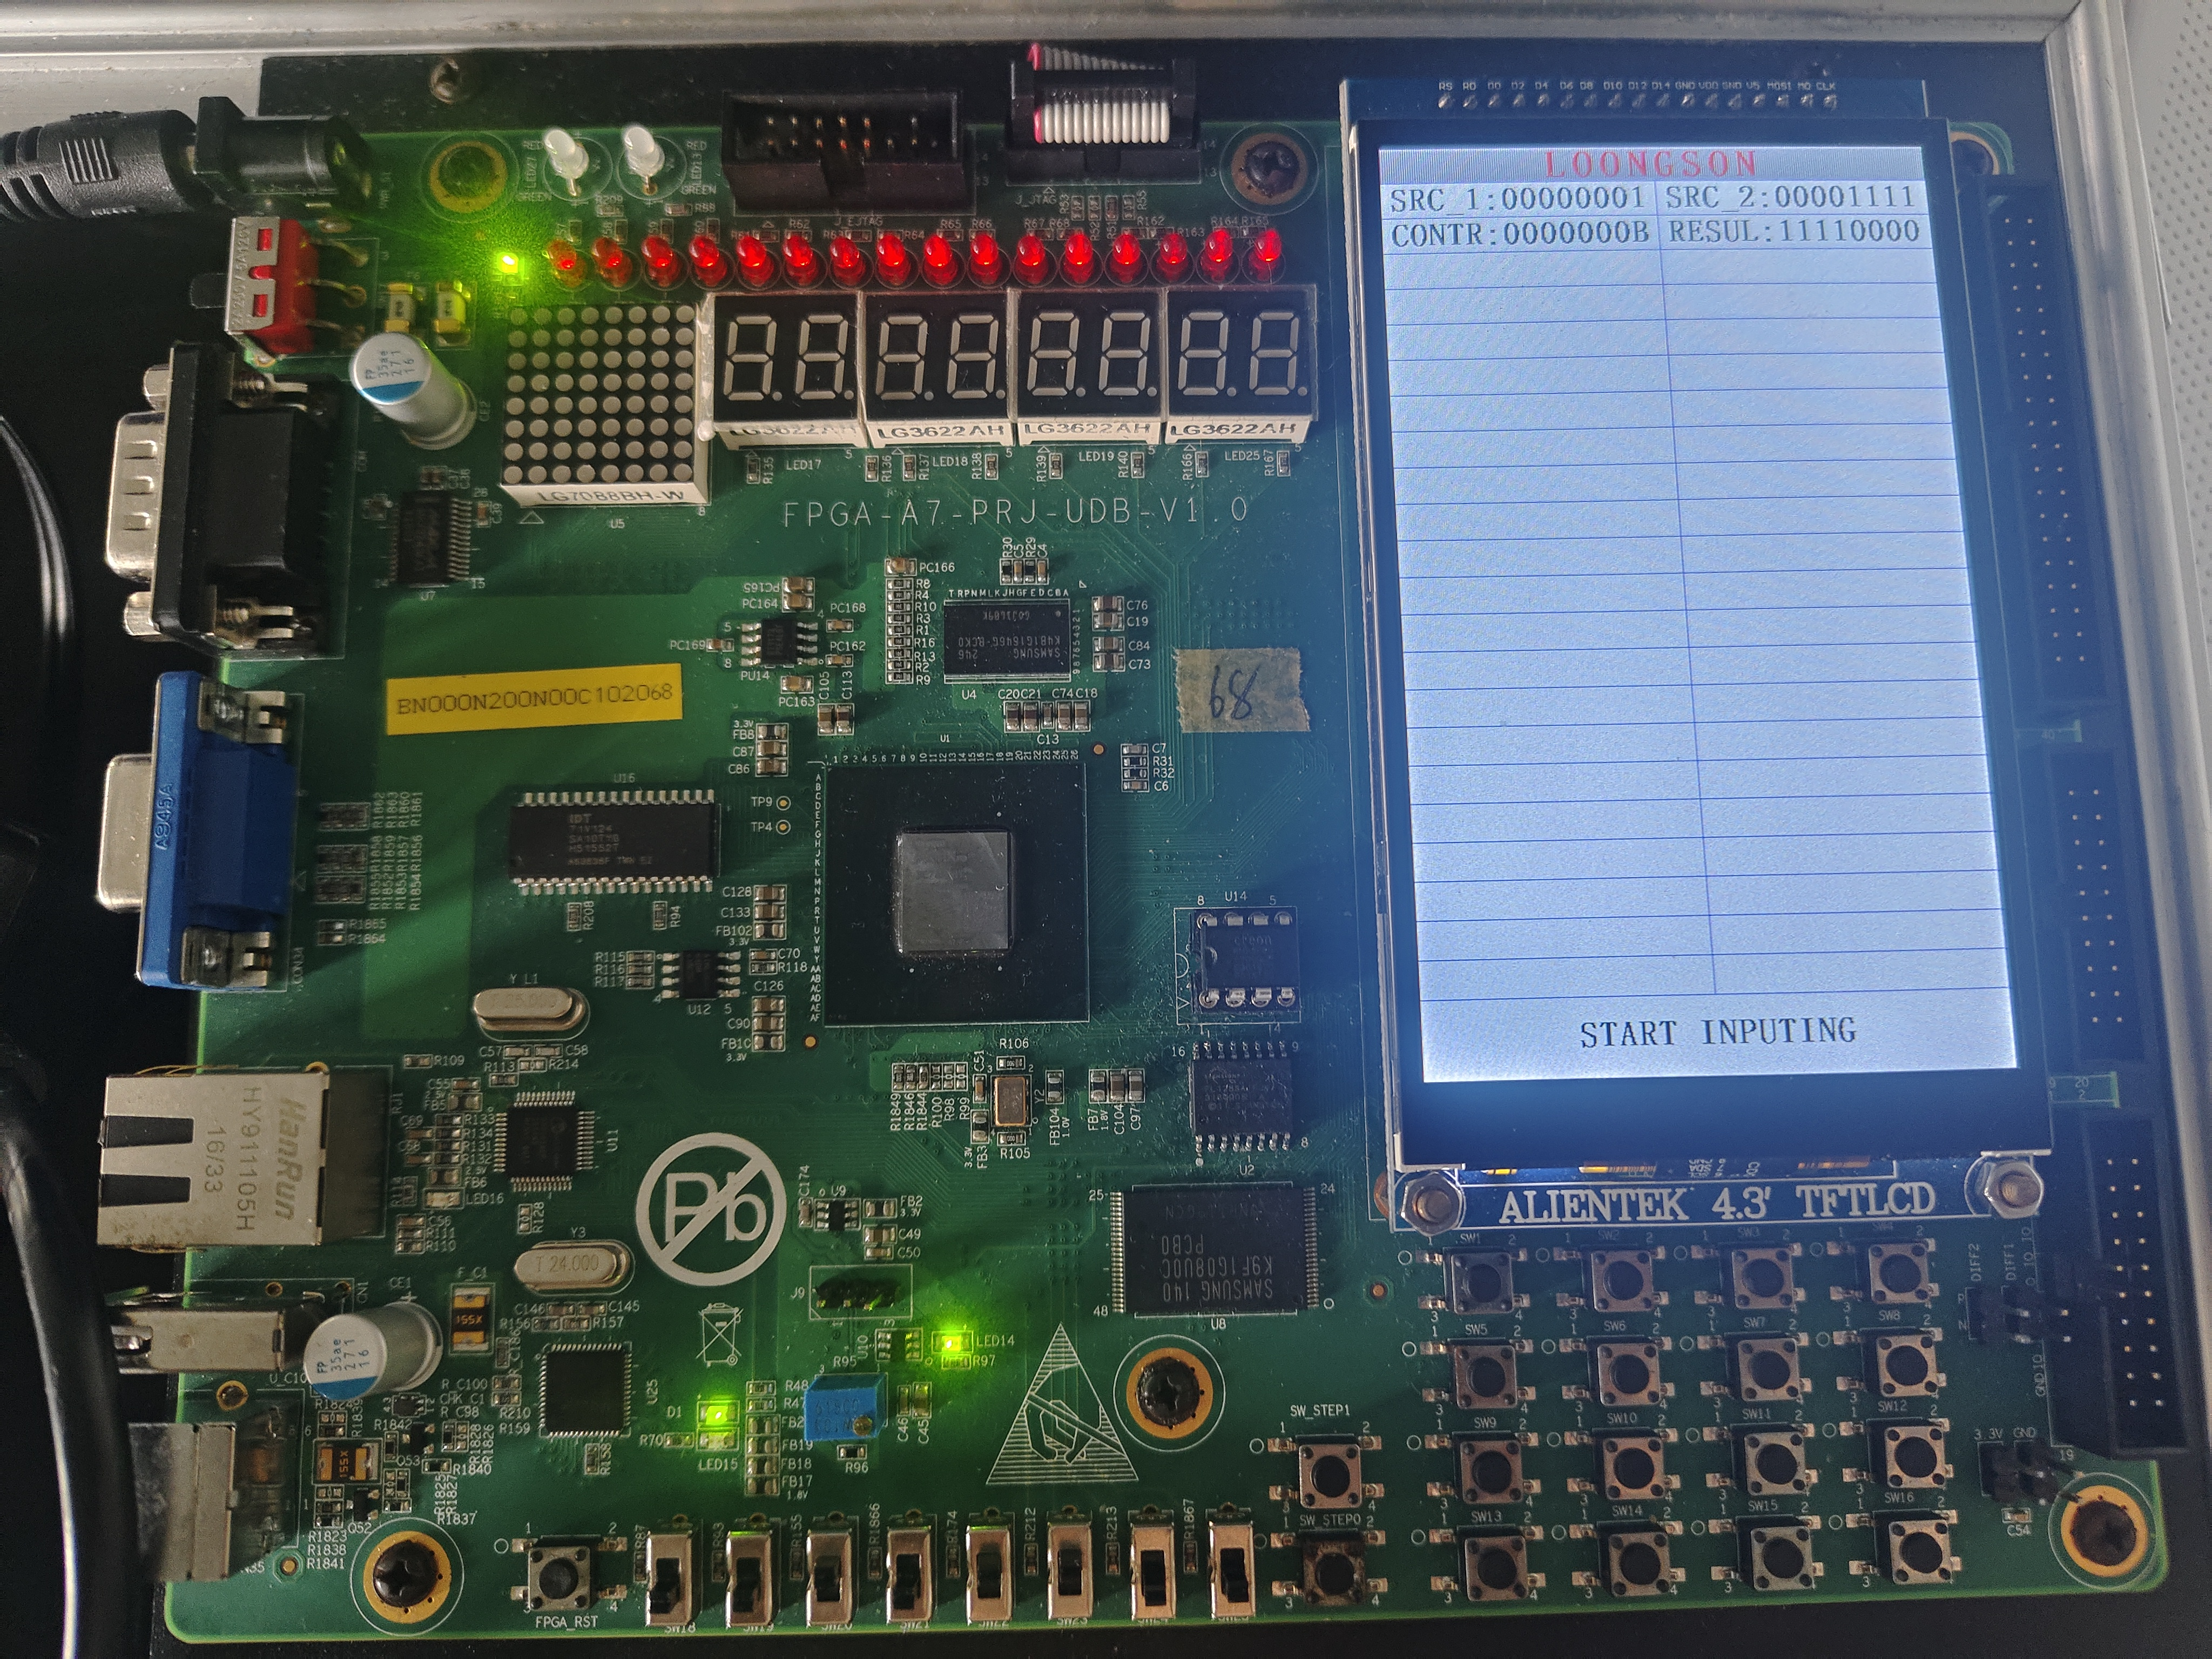
\includegraphics[width=\textwidth]{12.jpg}
    \caption{1011:LUI}
\end{figure}

\begin{figure}[h]
    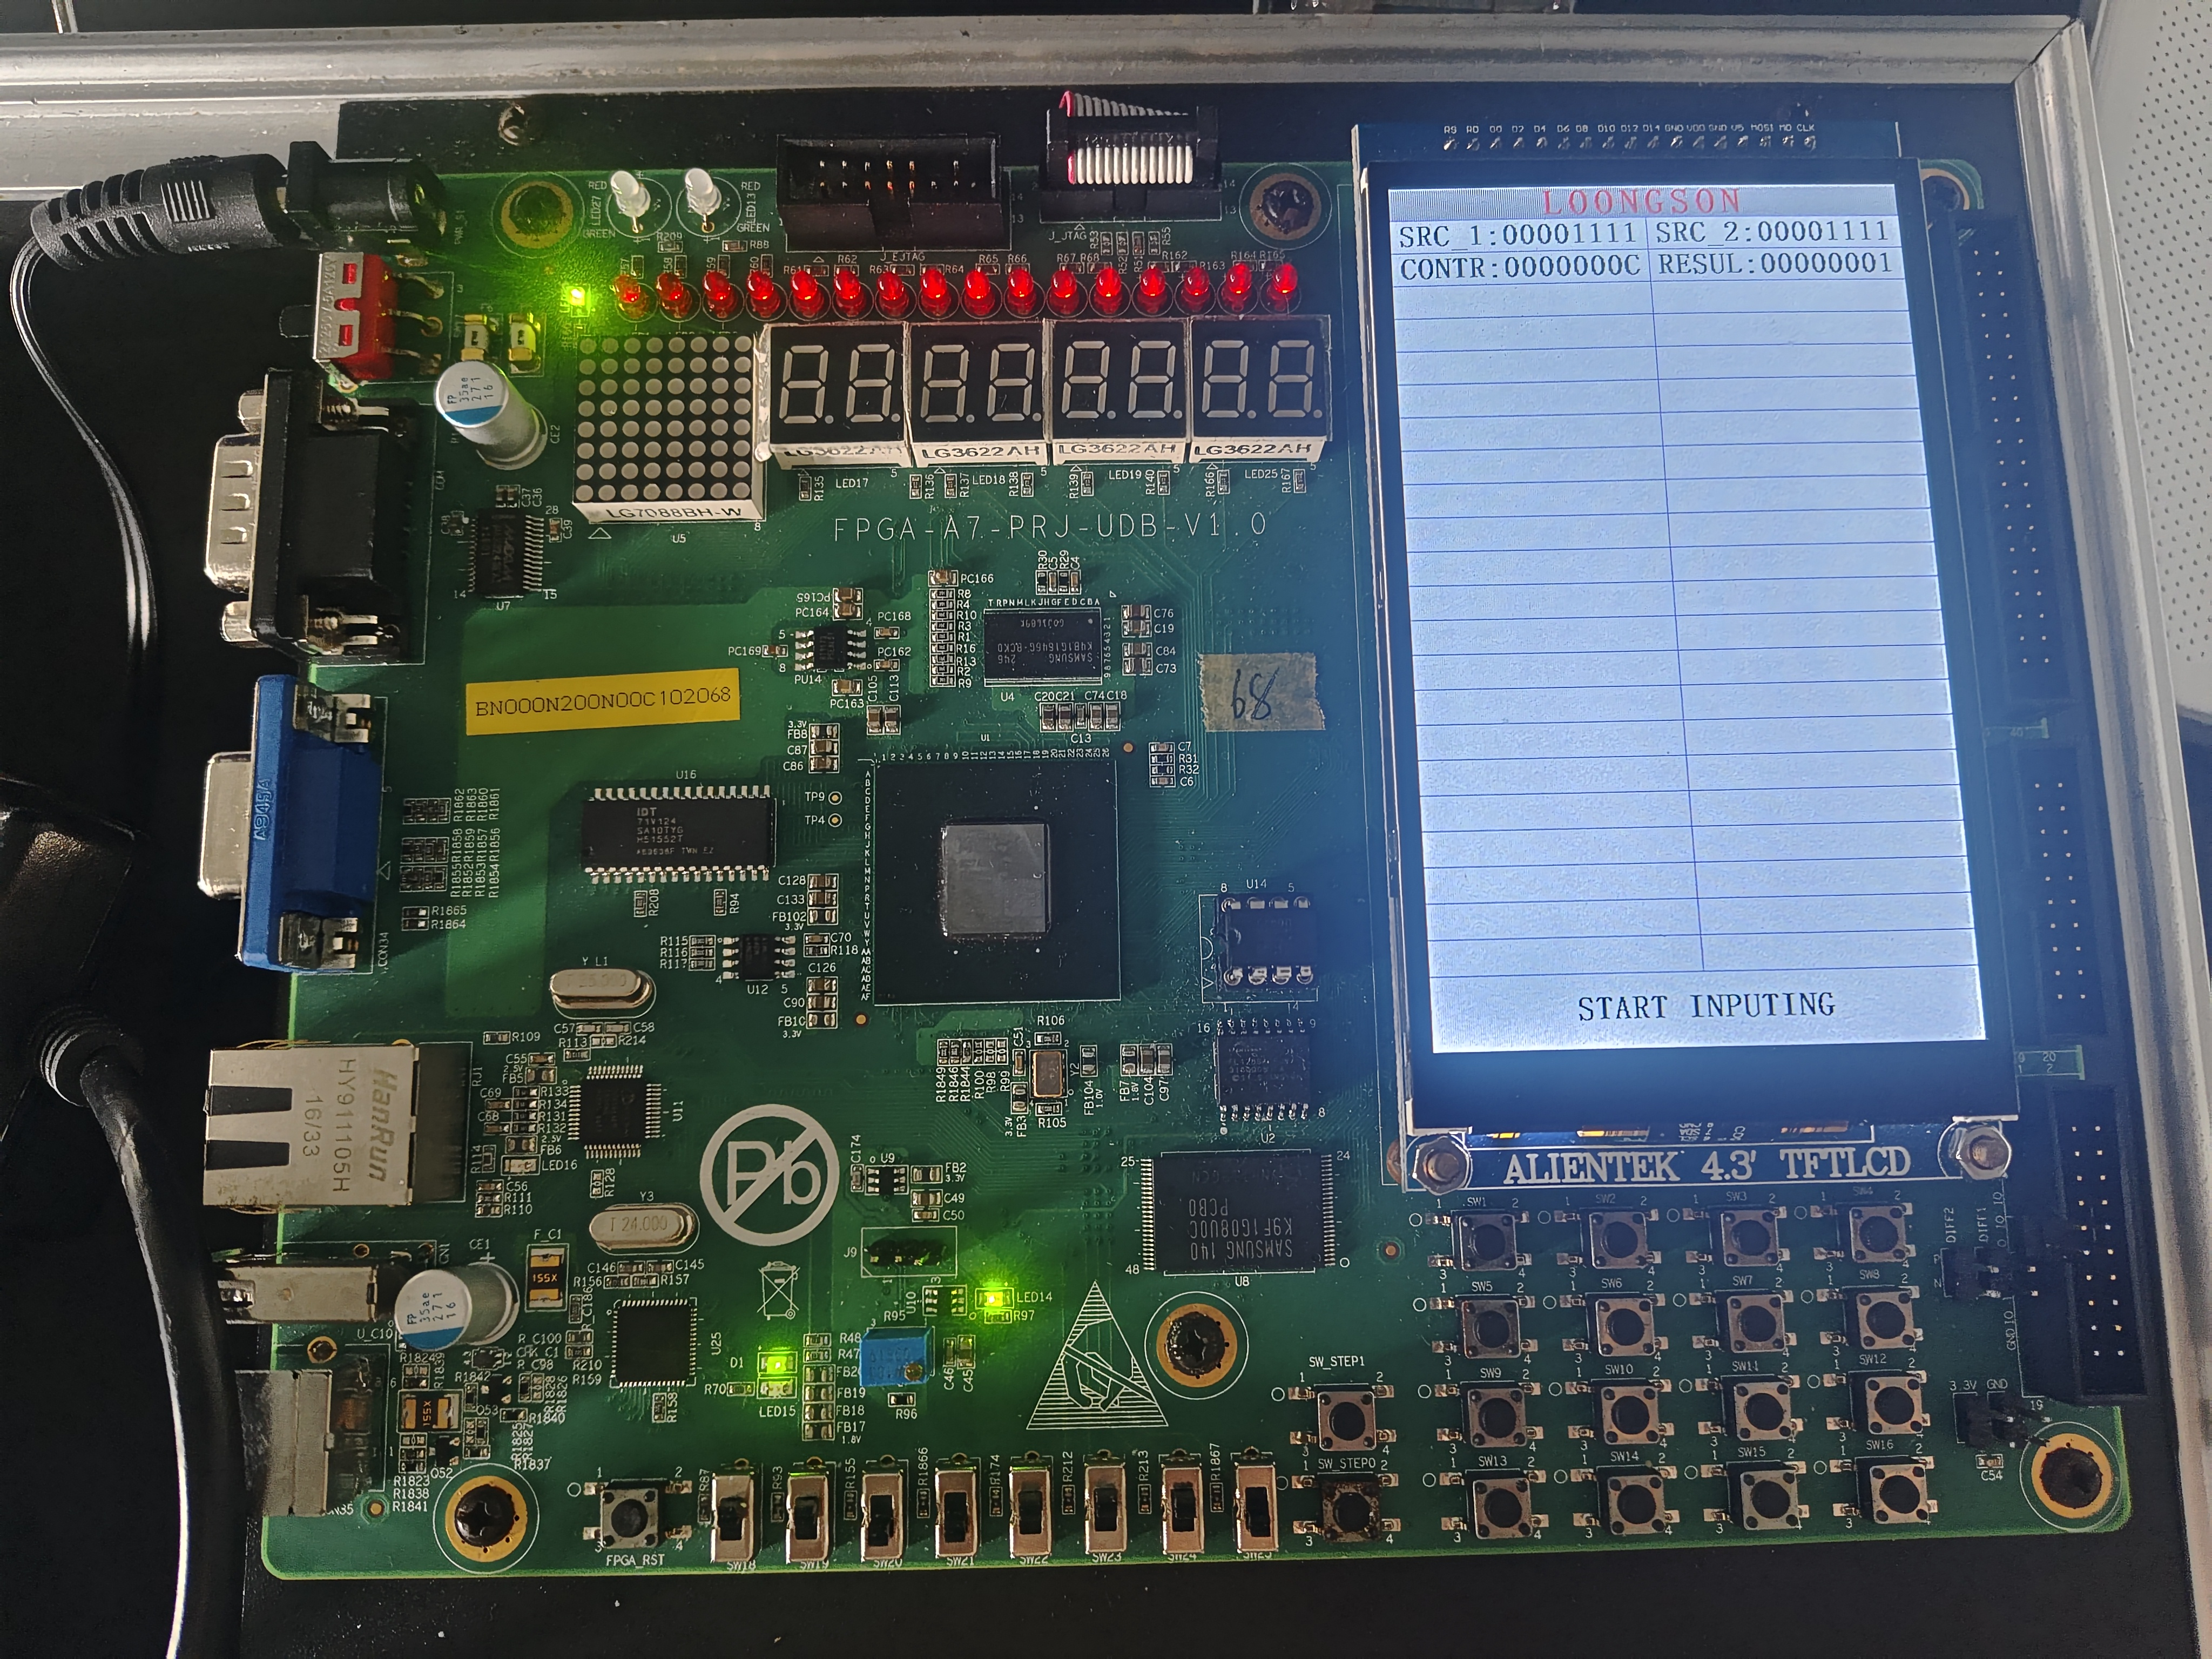
\includegraphics[width=\textwidth]{13.jpg}
    \caption{1100:SEQ}
\end{figure}

\begin{figure}[h]
    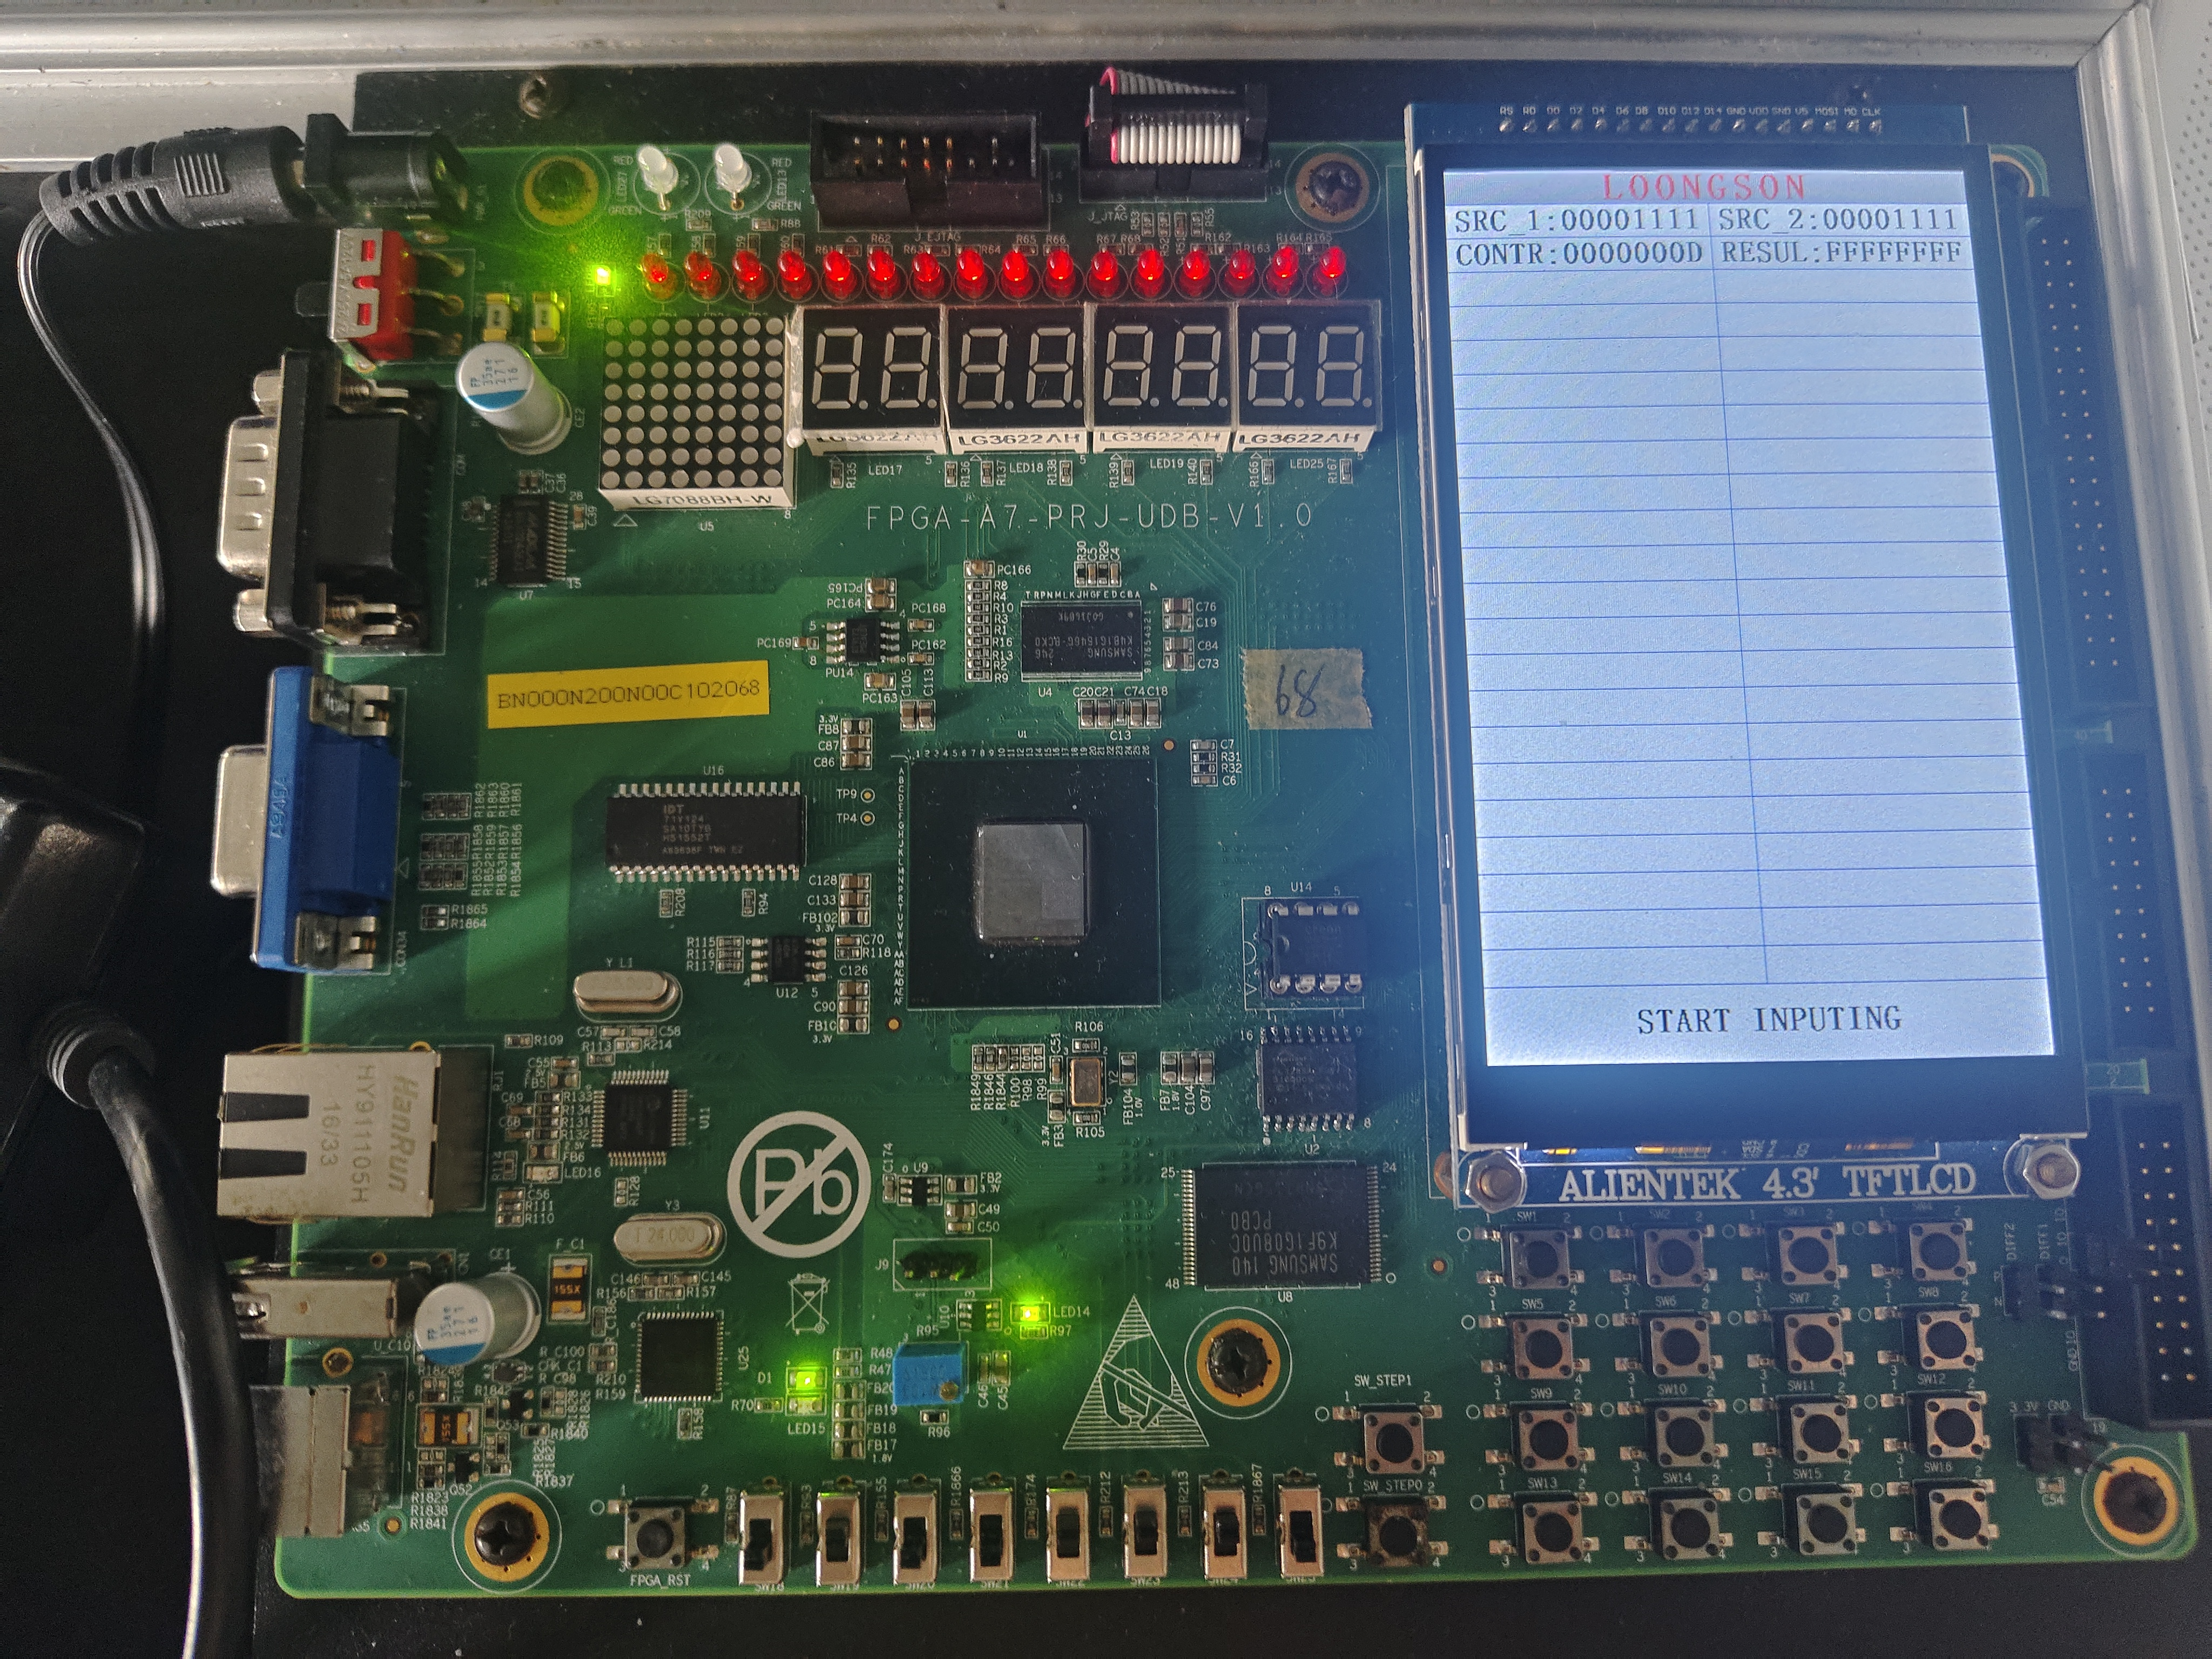
\includegraphics[width=\textwidth]{14.jpg}
    \caption{1101:XNOR}
\end{figure}

\begin{figure}[h]
    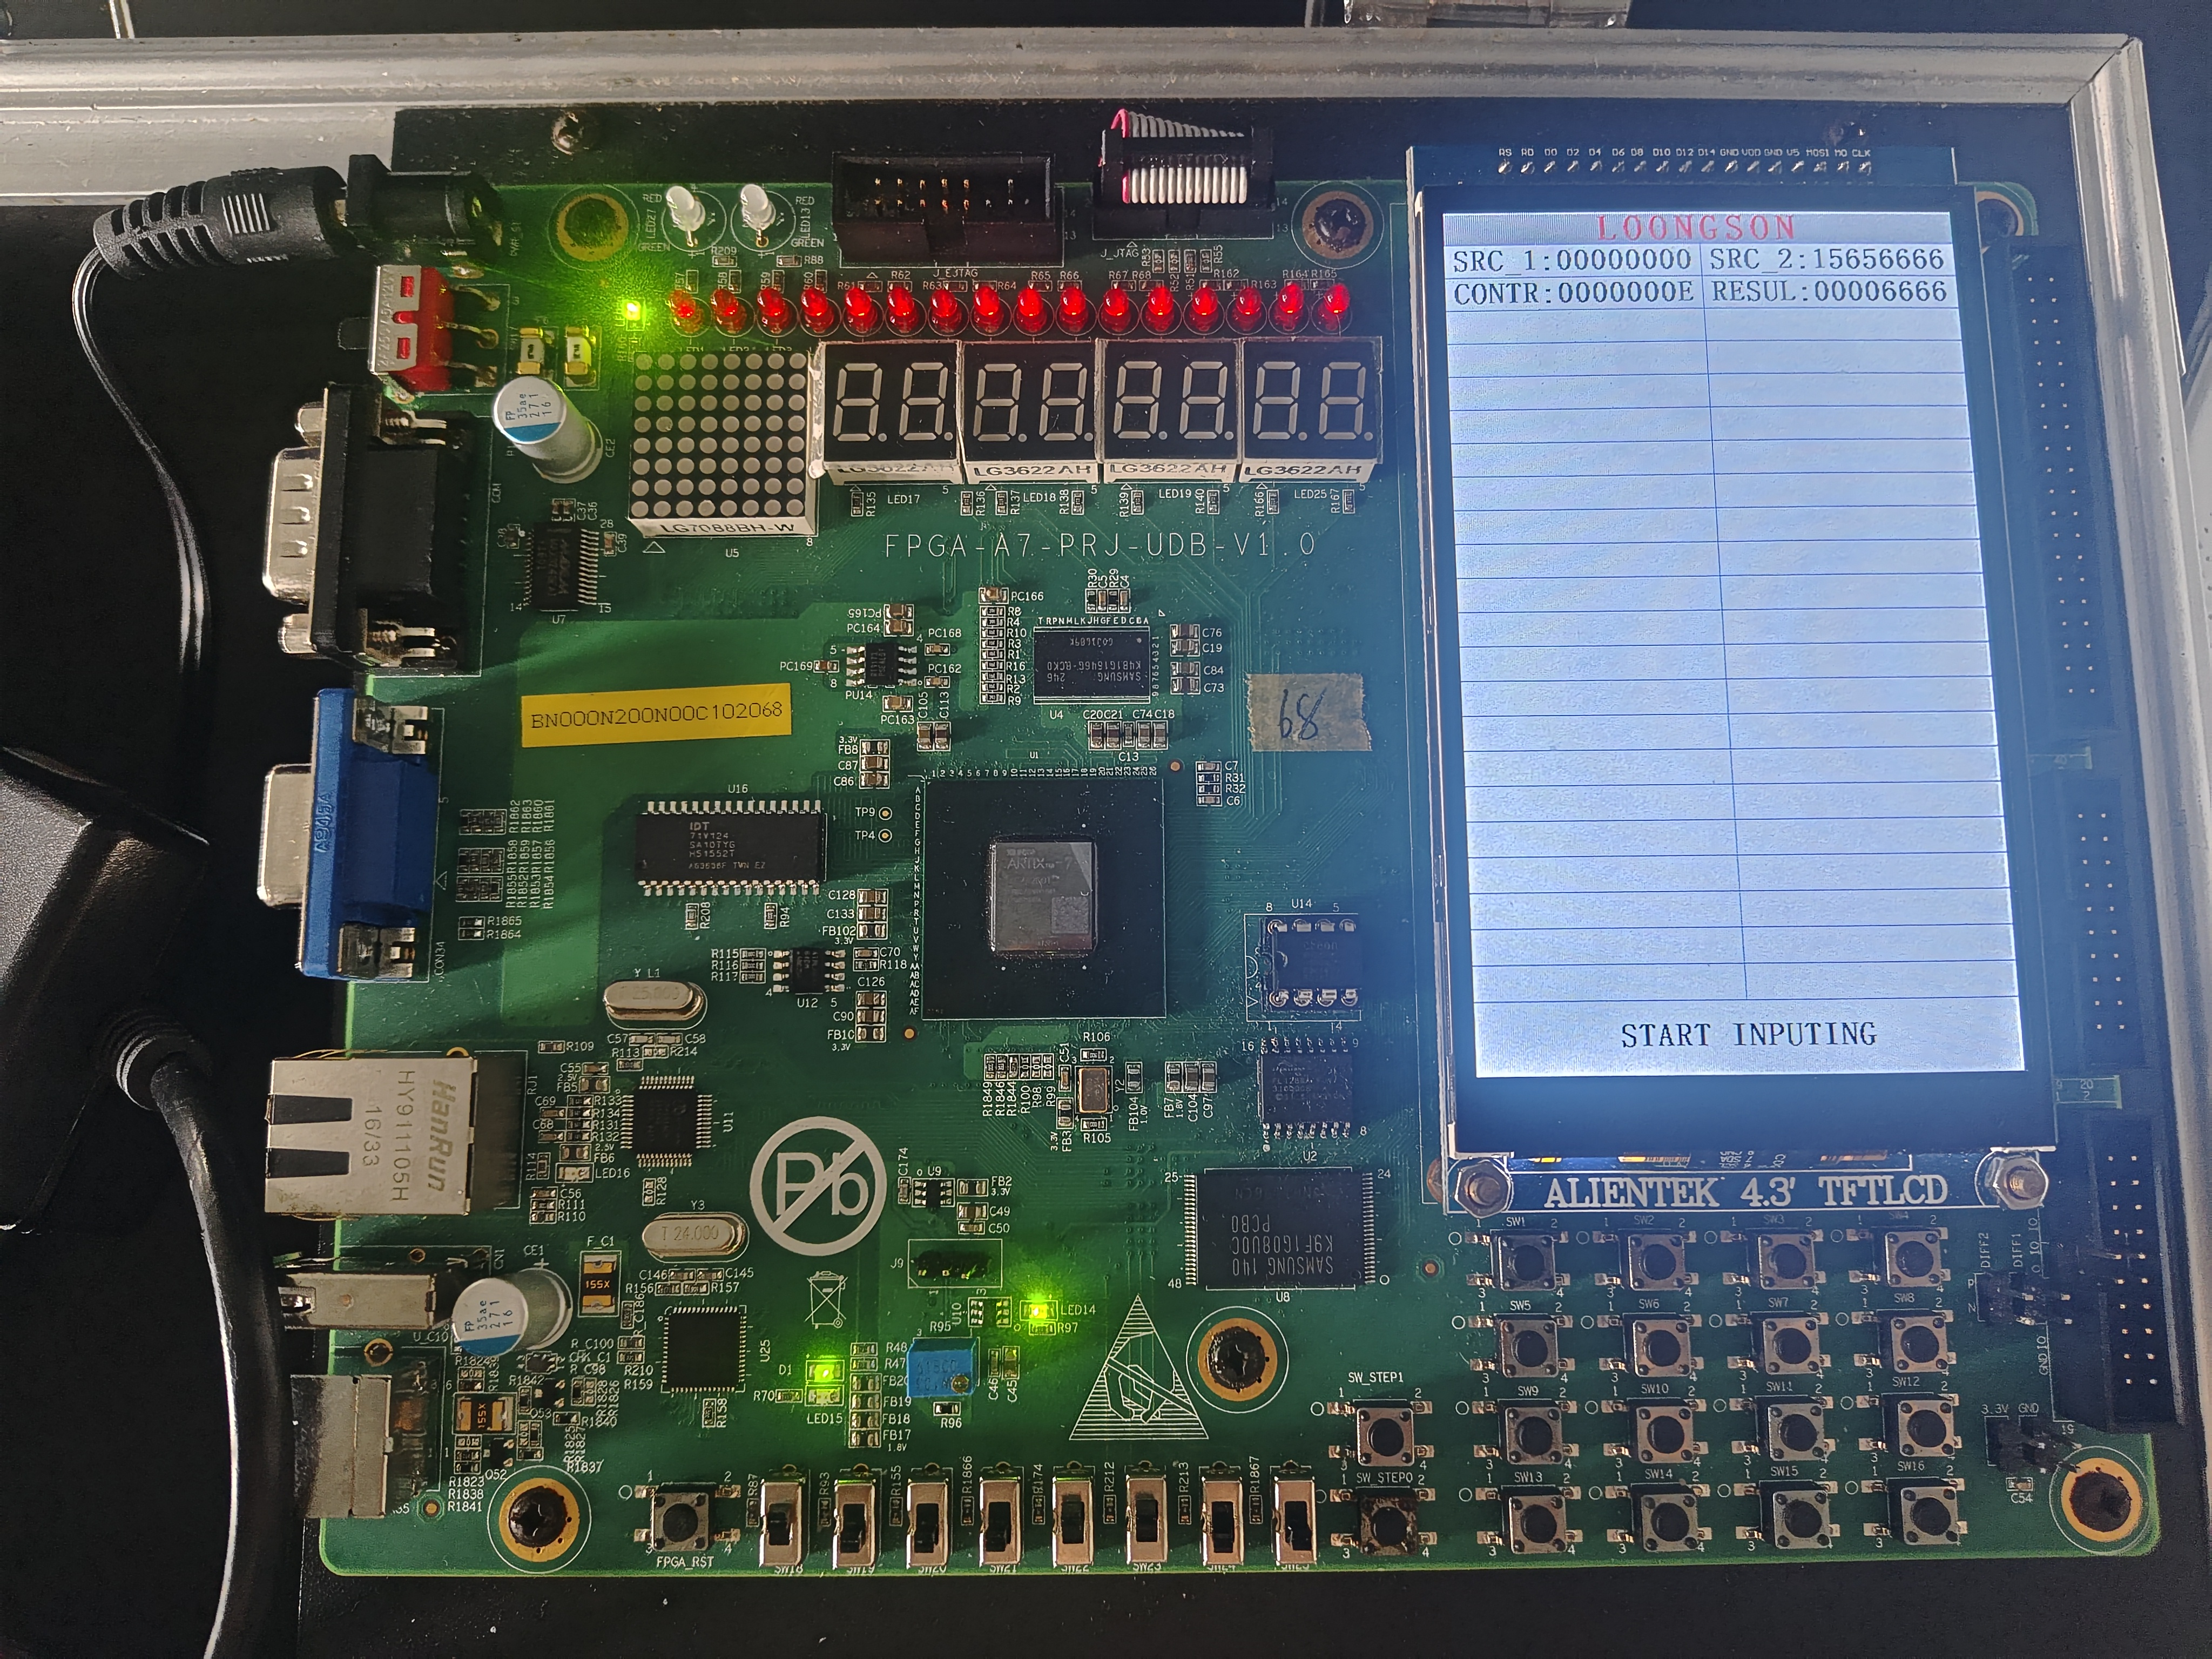
\includegraphics[width=\textwidth]{15.jpg}
    \caption{1110:LLI}
\end{figure}

\section{实验收获}
\begin{itemize}
   \item 熟悉了MIPS32指令集比较、位运算、加载等指令的具体实现
\end{itemize}

\section{附：源码目录}
\begin{itemize}
\item \verb|lab4/lab4.srcs/sources_1/new/adder.v|
\item \verb|lab4/lab4.srcs/sources_1/new/alu.v|
\item \verb|lab4/lab4.srcs/sources_1/new/alu_display.v|
\item \verb|lab4/lab4.srcs/constrs_1/new/alu.xdc|
\end{itemize}
\end{document}